% !TeX root = ../main.tex
% Copyright (c) 2026 Tyler Bignell
% Licensed under the MIT License - see LICENSE file for details

%%%%%%%%%%%%%%%%%%%%%%%%%%%%%%%%%%%%%%%%%%%%%%%%%%%%%%%%%%%
% CONDITIONALS & UTILITIES
%%%%%%%%%%%%%%%%%%%%%%%%%%%%%%%%%%%%%%%%%%%%%%%%%%%%%%%%%%%
\section{Conditionals \& Utilities}

	%%%%%%%%%%%%%%%%%%%%%%%%%%%%%%%%%%%%%%%%%%%%%%%%%%%%%%%%%%%
	\subsection{\texttt{xifthen}}
	\noindent\colorbox{themecolour!15}{\parbox{\linewidth}{\small This package is used internally by the template and is not typically invoked directly by the user.}}\vspace{0.5\baselineskip}
	
	The \texttt{xifthen} package lets the template make simple yes/no decisions based on your metadata settings in \texttt{main.tex}. For example, it checks whether \texttt{\textbackslash metaShowTodo} is set to \texttt{true} and shows or hides the todo list accordingly. You do not need to write any \texttt{xifthen} commands yourself, just set your metadata values and the template handles the rest.
	
	%%%%%%%%%%%%%%%%%%%%%%%%%%%%%%%%%%%%%%%%%%%%%%%%%%%%%%%%%%%
	\subsection{\texttt{xstring}}
	\noindent\colorbox{themecolour!15}{\parbox{\linewidth}{\small This package is used internally by the template for the smart header logic. Users do not use it directly.}}\vspace{0.5\baselineskip}
	
	The \texttt{xstring} package gives the template tools to read and work with text strings. The template uses it to check the length of \texttt{\textbackslash metaCourseName} and decide whether to show the full name or a shorter acronym in the header. The table below shows what \texttt{xstring} can do:
	
	\begin{tabularx}{\linewidth}{@{}lll@{}}
		\caption{Common \texttt{xstring} operations.}
		\label{tab:xstring} \\
		\toprule
		%%%%% HEADER ROW(S) %%%%%
		Operation & Command & Result \\
		\midrule
		\endfirsthead
		\toprule
		%%%%% HEADER ROW(S) %%%%%
		Operation & Command & Result \\
		\midrule
		\endhead
		\bottomrule
		\endfoot
		\bottomrule
		%%%%% NOTES %%%%%
		% NOTES HERE
		\endlastfoot
		%%%%% START %%%%%
		Extraction   & \texttt{\textbackslash StrLeft\{Lassonde\}\{4\}}       & \StrLeft{Lassonde}{4} \\
		
		Substitution & \texttt{\textbackslash StrSubstitute\{12/05/26\}\{/\}\{-\}} & \StrSubstitute{12/05/26}{/}{-} \\
		
		Length       & \texttt{\textbackslash StrLen\{YorkU\}}                & \StrLen{YorkU} \\
		
		Counting     & \texttt{\textbackslash StrCount\{Engineering\}\{n\}}   & \StrCount{Engineering}{n} \\
	\end{tabularx}
	
	%%%%%%%%%%%%%%%%%%%%%%%%%%%%%%%%%%%%%%%%%%%%%%%%%%%%%%%%%%%
	\subsection{\texttt{lipsum}}
	\noindent\colorbox{themecolour!15}{\parbox{\linewidth}{\small This package is used internally by the template for layout testing. It is not intended for use in final documents.}}\vspace{0.5\baselineskip}
	
	The \texttt{lipsum} package generates placeholder text for testing the layout and spacing of a page. Use \texttt{\textbackslash lipsum[n]} to generate paragraph $n$, or \texttt{\textbackslash lipsum[1-3]} to generate a range of paragraphs. The text is meaningless Latin and should be replaced with real content before submitting your document.
	
	An example of a paragraph of generated text:
	
	\lipsum[1]

%%%%%%%%%%%%%%%%%%%%%%%%%%%%%%%%%%%%%%%%%%%%%%%%%%%%%%%%%%%
% COLOURS
%%%%%%%%%%%%%%%%%%%%%%%%%%%%%%%%%%%%%%%%%%%%%%%%%%%%%%%%%%%
\section{Colours}

	%%%%%%%%%%%%%%%%%%%%%%%%%%%%%%%%%%%%%%%%%%%%%%%%%%%%%%%%%%%
	\subsection{\texttt{xcolor}}
	\noindent\colorbox{themecolour!15}{\parbox{\linewidth}{\small This package is used internally by the template for colour definitions and tints. Users may use it for custom colouring, but it is not required for normal document preparation.}}\vspace{0.5\baselineskip}
	
	The \texttt{xcolor} package adds colour support to \LaTeX. The template uses it to apply your chosen theme colour to headings, horizontal rules, boxes, and highlighted notes throughout the document.
	
		%%%%%%%%%%%%%%%%%%%%%%%%%%%%%%%%%%%%%%%%%%%%%%%%%%%%%%%%%%%
		\subsubsection{Setting the Theme Colour}
		You set the theme colour by editing \texttt{\textbackslash metaThemeColour} in \texttt{main.tex}. You can type a hex colour code, the name of any built-in colour, or the name of a custom colour defined in the template. If you leave it empty, the template uses \texttt{DefaultBlue}.
		
		\begin{tabularx}{\linewidth}{@{}lll@{}}
			\caption{Accepted values for \texttt{\textbackslash metaThemeColour}.}
				\label{tab:theme-colour-values} \\
			\toprule
			%%%%% HEADER ROW(S) %%%%%
			Type & Example Value & Effect \\
			\midrule
			\endfirsthead
			\toprule
			%%%%% HEADER ROW(S) %%%%%
			Type & Example Value & Effect \\
			\midrule
			\endhead
			\bottomrule
			\endfoot
			\bottomrule
			%%%%% NOTES %%%%%
			% NOTES HERE
			\endlastfoot
			%%%%% START %%%%%
			Empty         & \texttt{}        & Defaults to \texttt{DefaultBlue} \\
			
			Hex code      & \texttt{\#810001}  & Parsed as an HTML hex colour \\
			
			Named colour  & \texttt{red}     & Resolved via \texttt{\textbackslash colorlet} \\
			
			Custom colour & \texttt{LassondeNavy} & Any colour defined in the sty file \\
		\end{tabularx}
		
		The same applies to \texttt{\textbackslash metaLinkColour}, \texttt{\textbackslash metaCiteColour}, and \texttt{\textbackslash metaUrlColour}; each one also falls back to \texttt{themecolour} when left empty.
		
		%%%%%%%%%%%%%%%%%%%%%%%%%%%%%%%%%%%%%%%%%%%%%%%%%%%%%%%%%%%
		\subsubsection{Custom Defined Colours}
		These colours are built into the template and can be typed directly into \texttt{\textbackslash metaThemeColour} or any colour command:
		
		\begin{tabularx}{\linewidth}{@{}lcc@{}}
			\caption{Custom colours defined in \texttt{stemtemplate.sty}.}
			\label{tab:custom-colours} \\
			\toprule
			%%%%% HEADER ROW(S) %%%%%
			Name & Hex & Preview \\
			\midrule
			\endfirsthead
			\toprule
			%%%%% HEADER ROW(S) %%%%%
			Name & Hex & Preview \\
			\midrule
			\endhead
			\bottomrule
			\endfoot
			\bottomrule
			%%%%% NOTES %%%%%
			\multicolumn{3}{l}{{\footnotesize \textsuperscript{a} Unaffiliated professional blue.}} \\
			\multicolumn{3}{l}{{\footnotesize \textsuperscript{b} Recommended for York U Faculty of Science students.}} \\
			\multicolumn{3}{l}{{\footnotesize \textsuperscript{c} Recommended for York U Lassonde students.}} \\
			\endlastfoot
			%%%%% START %%%%%
			\texttt{DefaultBlue} \textsuperscript{a} & \texttt{\#1B4F8A} & \textcolor{white}{\colorbox{DefaultBlue}{\phantom{XXXXX}}}  \\
			
			\texttt{YorkRedDark} & \texttt{\#810001} & \textcolor{white}{\colorbox{YorkRedDark}{\phantom{XXXXX}}}     \\
			
			\texttt{ScienceSkyBlueDark} \textsuperscript{b} & \texttt{\#065C87} & \textcolor{white}{\colorbox{ScienceSkyBlueDark}{\phantom{XXXXX}}}  \\
			
			\texttt{LassondeNavy} \textsuperscript{c} & \texttt{\#003366} & \textcolor{white}{\colorbox{LassondeNavy}{\phantom{XXXXX}}} \\
		\end{tabularx}
		
		%%%%%%%%%%%%%%%%%%%%%%%%%%%%%%%%%%%%%%%%%%%%%%%%%%%%%%%%%%%
		\subsubsection{Built-in Named Colours}
		You can also use any of \texttt{xcolor}'s built-in colour names. A small selection is shown below. For the full list, see \url{https://mirrors.ctan.org/macros/latex/contrib/xcolor/xcolor.pdf}:
		
		\begin{tabularx}{\linewidth}{@{}lcclc@{}}
			\caption{Built-in \texttt{xcolor} named colours.}
			\label{tab:named-colours} \\
			\toprule
			%%%%% HEADER ROW(S) %%%%%
			Name & Preview & \ & Name & Preview \\
			\midrule
			\endfirsthead
			\toprule
			%%%%% HEADER ROW(S) %%%%%
			Name & Preview & \ & Name & Preview \\
			\midrule
			\endhead
			\bottomrule
			\endfoot
			\bottomrule
			%%%%% NOTES %%%%%
			% NOTES HERE
			\endlastfoot
			%%%%% START %%%%%
			\multicolumn{5}{c}{\textit{Base colours}} \\
			
			\texttt{red}       	 & \colorbox{red}{\phantom{XXXXX}}       			& & \texttt{cyan}      	 & \colorbox{cyan}{\phantom{XXXXX}}      \\
			
			\texttt{green}     	 & \colorbox{green}{\phantom{XXXXX}}     			& & \texttt{magenta}     & \colorbox{magenta}{\phantom{XXXXX}}      \\
			
			\texttt{blue}   	 & \colorbox{blue}{\phantom{XXXXX}}   				& & \texttt{yellow}    	 & \colorbox{yellow}{\phantom{XXXXX}}    \\
			
			\texttt{black}     	 & \colorbox{black}{\phantom{XXXXX}}     			& & \texttt{white}     	 & \colorbox{white}{\phantom{XXXXX}}     \\
			
			\texttt{gray}  		 & \colorbox{gray}{\phantom{XXXXX}}  				& & \texttt{brown}       & \colorbox{brown}{\phantom{XXXXX}}      \\
			
			\midrule
			
			\multicolumn{5}{c}{\textit{Extended colour sets (dvipsnames, svgnames, x11names})} \\
			
			\texttt{NavyBlue}    & \colorbox{NavyBlue}{\phantom{XXXXX}}      		& & \texttt{ForestGreen} & \colorbox{ForestGreen}{\phantom{XXXXX}}     \\
			
			\texttt{Maroon}    	 & \colorbox{Maroon}{\phantom{XXXXX}}    			& & \texttt{BurntOrange} & \colorbox{BurntOrange}{\phantom{XXXXX}}      \\
			
			\texttt{RoyalPurple} & \colorbox{RoyalPurple}{\phantom{XXXXX}}    		& & \texttt{Sepia}       & \colorbox{Sepia}{\phantom{XXXXX}}      \\
			
			\texttt{SlateGray}   & \colorbox{SlateGray}{\phantom{XXXXX}}    		& & \texttt{Teal}     	 & \colorbox{Teal}{\phantom{XXXXX}}     \\
			
			\texttt{SteelBlue4}	 & \colorbox{SteelBlue4}{\phantom{XXXXX}} 			& & \texttt{Firebrick3}  & \colorbox{Firebrick3}{\phantom{XXXXX}}     \\
		\end{tabularx}
		
		%%%%%%%%%%%%%%%%%%%%%%%%%%%%%%%%%%%%%%%%%%%%%%%%%%%%%%%%%%%
		\subsubsection{Theme Colour and Tints}
		Adding \texttt{!} followed by a number after any colour name creates a lighter version of that colour, called a \textit{tint}. The number is the percentage of the original colour, so \texttt{themecolour!75} is 75\% colour and 25\% white.
		
		You can extend this to mix with any second colour, not just white, by adding a second \texttt{!} and colour name: \texttt{colourA!X!colourB} gives \(X\%\) \texttt{colourA} blended with \((100-X)\%\) \texttt{colourB}. Mixing toward \texttt{black} instead of white produces a \textit{shade} rather than a tint, and mixing toward any other colour produces a custom blend:
		
		\begin{tabularx}{\linewidth}{@{}llc@{}}
			\caption{Active theme colour, tints, shades, and blends.}
			\label{tab:tints} \\
			\toprule
			%%%%% HEADER ROW(S) %%%%%
			Name & Mix & Preview \\
			\midrule
			\endfirsthead
			\toprule
			%%%%% HEADER ROW(S) %%%%%
			Name & Mix & Preview \\
			\midrule
			\endhead
			\bottomrule
			\endfoot
			\bottomrule
			%%%%% NOTES %%%%%
			% NOTES HERE
			\endlastfoot
			%%%%% START %%%%%
			
			% TINTS (toward white)
			\multicolumn{3}{c}{\textit{Tints --- blended toward white}} \\
			
			\texttt{themecolour}     & 100\% colour & \textcolor{white}{\colorbox{themecolour}{\phantom{XXXXX}}} \\
			
			\texttt{themecolour!75}  & 75\% colour  & \textcolor{white}{\colorbox{themecolour!75}{\phantom{XXXXX}}} \\
			
			\texttt{themecolour!50}  & 50\% colour  & \colorbox{themecolour!50}{\phantom{XXXXX}} \\
			
			\texttt{themecolour!25}  & 25\% colour  & \colorbox{themecolour!25}{\phantom{XXXXX}} \\
			
			\midrule
			
			% SHADES (toward black)
			\multicolumn{3}{c}{\textit{Shades --- blended toward black}} \\
			
			\texttt{themecolour!100!black} & 100\% colour, 0\% black & \colorbox{themecolour!100!black}{\phantom{XXXXX}} \\
			
			\texttt{themecolour!75!black}  & 75\% colour, 25\% black & \colorbox{themecolour!75!black}{\phantom{XXXXX}} \\
			
			\texttt{themecolour!50!black}  & 50\% colour, 50\% black & \colorbox{themecolour!50!black}{\phantom{XXXXX}} \\
			
			\texttt{themecolour!25!black}  & 25\% colour, 75\% black & \colorbox{themecolour!25!black}{\phantom{XXXXX}} \\
			
			\midrule
			
			% BLENDS (toward another hue)
			\multicolumn{3}{c}{\textit{Blends --- toward another colour}} \\
			
			\texttt{themecolour!70!cyan}    & 70\% colour, 30\% cyan    & \colorbox{themecolour!70!cyan}{\phantom{XXXXX}} \\
			
			\texttt{themecolour!70!magenta} & 70\% colour, 30\% magenta & \colorbox{themecolour!70!magenta}{\phantom{XXXXX}} \\
			
			\texttt{themecolour!70!yellow}  & 70\% colour, 30\% yellow  & \colorbox{themecolour!70!yellow}{\phantom{XXXXX}} \\
			
			\texttt{themecolour!70!red}  	& 70\% colour, 30\% red  	& \colorbox{themecolour!70!red}{\phantom{XXXXX}} \\
			
			\texttt{themecolour!70!green}   & 70\% colour, 30\% green   & \colorbox{themecolour!75!green}{\phantom{XXXXX}} \\
			
			\texttt{themecolour!70!blue}  	& 70\% colour, 30\% blue  	& \colorbox{themecolour!70!blue}{\phantom{XXXXX}} \\
		\end{tabularx}
		
		%%%%%%%%%%%%%%%%%%%%%%%%%%%%%%%%%%%%%%%%%%%%%%%%%%%%%%%%%%%
		\subsubsection{Using \texttt{\textbackslash textcolor} and \texttt{\textbackslash colorbox}}
		Use \texttt{\textbackslash textcolor} to change the colour of a word or phrase in your text. It takes two arguments: the colour name and the text to colour. For example, \textcolor{themecolour}{\texttt{\textbackslash textcolor\{themecolour\}\{Sample Text\}}} colours the text without changing anything else on the line.
		
		Use \texttt{\textbackslash colorbox} to place a coloured background behind text, useful for drawing attention to a short note or label. For example, \colorbox{themecolour!15}{\texttt{\textbackslash colorbox\{themecolour!15\}\{Sample Text\}}} produces a lightly shaded highlight box.

%%%%%%%%%%%%%%%%%%%%%%%%%%%%%%%%%%%%%%%%%%%%%%%%%%%%%%%%%%%
% PAGE GEOMETRY
%%%%%%%%%%%%%%%%%%%%%%%%%%%%%%%%%%%%%%%%%%%%%%%%%%%%%%%%%%%
\section{Page Geometry}

	%%%%%%%%%%%%%%%%%%%%%%%%%%%%%%%%%%%%%%%%%%%%%%%%%%%%%%%%%%%
	\subsection{\texttt{geometry}}
	\noindent\colorbox{themecolour!15}{\parbox{\linewidth}{\small This package is used internally by the template to configure page margins and layout. Users do not normally modify these settings.}}\vspace{0.5\baselineskip}
	
	The \texttt{geometry} package controls the page margins and the size of the text area. The template uses it to set standard margins automatically, you do not need to touch anything for your document to be formatted correctly.
	
	%%%%%%%%%%%%%%%%%%%%%%%%%%%%%%%%%%%%%%%%%%%%%%%%%%%%%%%%%%%
	\subsection{\texttt{setspace}}
	\noindent\colorbox{themecolour!15}{\parbox{\linewidth}{\small This package is used internally by the template to control line spacing. Users normally do not interact with it directly, but spacing can be adjusted through metadata commands in \texttt{main.tex}.}}\vspace{0.5\baselineskip}
	
	The \texttt{setspace} package controls the space between lines of text. You can choose between single, one-and-a-half, or double spacing by setting the appropriate metadata value in \texttt{main.tex}, you do not need to call any \texttt{setspace} commands yourself.
	
	%%%%%%%%%%%%%%%%%%%%%%%%%%%%%%%%%%%%%%%%%%%%%%%%%%%%%%%%%%%
	\begin{landscape} 	  % Begins landscape
	\thispagestyle{plain} % Removes header from landscape page
	\subsection{\texttt{pdflscape}}
	\noindent\colorbox{themecolour!15}{\parbox{\linewidth}{\small This package is available for rotating wide tables or figures into landscape orientation. It is not required for normal document preparation and is only used when the author explicitly includes a landscape environment.}}\vspace{0.5\baselineskip}
	
	The \texttt{pdflscape} package lets you rotate a page sideways so that wide content fits. Wrap anything in a \texttt{landscape} environment and that page will display in landscape orientation in the PDF viewer. The page after it returns to portrait automatically.
	
	The table below is an example of content that is too wide for portrait and benefits from a landscape page:
	
	\begin{tabularx}{\linewidth}{@{}LCCCCC@{}}
		\caption{Wide data table spanning landscape page.}
		\label{tab:landscape} \\
		\toprule
		%%%%% HEADER ROW(S) %%%%%
		Parameter & Trial 1 & Trial 2 & Trial 3 & Trial 4 & Trial 5 \\
		\midrule
		\endfirsthead
		\toprule
		%%%%% HEADER ROW(S) %%%%%
		Parameter & Trial 1 & Trial 2 & Trial 3 & Trial 4 & Trial 5 \\
		\midrule
		\endhead
		\bottomrule
		\endfoot
		\bottomrule
		%%%%% NOTES %%%%%
		% NOTES HERE
		\endlastfoot
		%%%%% START %%%%%
		Temperature (\si{\celsius})     & 23.4 & 24.1 & 22.8 & 23.9 & 24.5 \\
		
		Pressure (\si{\kilo\pascal})  & 101.3 & 101.1 & 101.5 & 100.9 & 101.4 \\
		
		Humidity (\%)               & 48.7 & 50.2 & 47.9 & 51.0 & 49.3 \\
		
		Voltage (\si{\volt})          & 4.98 & 5.01 & 4.97 & 5.02 & 5.00 \\
		
		Current (\si{\milli\ampere}) & 120.1 & 119.8 & 120.4 & 120.0 & 119.6 \\
	\end{tabularx}
	
	Use \texttt{$\backslash$thispagestyle\{plain\}} on the line after \texttt{$\backslash$begin\{landscape\}} to remove the header from the rotated page. Use \texttt{$\backslash$thispagestyle\{empty\}} instead if you also want to hide the page number in the footer.
	\end{landscape} % Ends landscape

%%%%%%%%%%%%%%%%%%%%%%%%%%%%%%%%%%%%%%%%%%%%%%%%%%%%%%%%%%%
% LANGUAGE & FONT
%%%%%%%%%%%%%%%%%%%%%%%%%%%%%%%%%%%%%%%%%%%%%%%%%%%%%%%%%%%
\section{Language \& Font}

	%%%%%%%%%%%%%%%%%%%%%%%%%%%%%%%%%%%%%%%%%%%%%%%%%%%%%%%%%%%
	\subsection{\texttt{babel}}
	\noindent\colorbox{themecolour!15}{\parbox{\linewidth}{\small This package manages language-specific typographic rules. The template loads it automatically with English as the active language.}}\vspace{0.5\baselineskip}
	
	The \texttt{babel} package tells \LaTeX{} which language the document is written in. The template loads it with English so that words are hyphenated correctly and punctuation follows English conventions. No changes are needed on your end.
	
	%%%%%%%%%%%%%%%%%%%%%%%%%%%%%%%%%%%%%%%%%%%%%%%%%%%%%%%%%%%
	\subsection{\texttt{fontspec}}
	\noindent\colorbox{themecolour!15}{\parbox{\linewidth}{\small This package provides system font access under XeLaTeX. It is loaded automatically by the template.}}\vspace{0.5\baselineskip}
	
	The \texttt{fontspec} package is the foundation of font loading under Xe\LaTeX{}. It allows the template to load any font installed on your system by name, and handles all character encoding internally. You do not need to configure it; the template applies it automatically based on your metadata.
	
		%%%%%%%%%%%%%%%%%%%%%%%%%%%%%%%%%%%%%%%%%%%%%%%%%%%%%%%%%%%
		\subsubsection{\texttt{\textbackslash metaSerifFont} and \texttt{\textbackslash seriftext}}
		\noindent\colorbox{themecolour!15}{\parbox{\linewidth}{\small The serif font is configured through metadata. Users typically only use the \texttt{\textbackslash seriftext\{\}} command directly.}}\vspace{0.5\baselineskip}
		
		The \texttt{\textbackslash metaSerifFont} metadata key sets the serif font for the document. Leave it empty to use the default, IBM Plex Serif. To override it, set it to any font installed on your system by exact name, for example \texttt{Georgia} or \texttt{Times New Roman}.
		
		Use \texttt{\textbackslash seriftext\{\}} to apply the serif font to a specific word or phrase regardless of which font the document body is using:
		
		\seriftext{This text is rendered in the serif font.}
		
		%%%%%%%%%%%%%%%%%%%%%%%%%%%%%%%%%%%%%%%%%%%%%%%%%%%%%%%%%%%
		\subsubsection{\texttt{\textbackslash metaSansFont} and \texttt{\textbackslash sansseriftext}}
		\noindent\colorbox{themecolour!15}{\parbox{\linewidth}{\small The sans-serif font is configured through metadata. Users normally interact with it only through \texttt{\textbackslash sansseriftext\{\}}.}}\vspace{0.5\baselineskip}
		
		The \texttt{\textbackslash metaSansFont} metadata key sets the sans-serif font for the document. Leave it empty to use the default, IBM Plex Sans. To override it, set it to any font installed on your system by exact name, for example \texttt{Arial} or \texttt{Helvetica Neue}.
		
		Use \texttt{\textbackslash sansseriftext\{\}} to apply the sans-serif font to a specific word or phrase:
		
		\sansseriftext{This text is rendered in the sans-serif font.}
		
		%%%%%%%%%%%%%%%%%%%%%%%%%%%%%%%%%%%%%%%%%%%%%%%%%%%%%%%%%%%
		\subsubsection{Default Font}
		\noindent\colorbox{themecolour!15}{\parbox{\linewidth}{\small The template selects the global font through the metadata in \texttt{main.tex}; users do not modify font packages directly.}}\vspace{0.5\baselineskip}
		
		You control which font family the document body uses by setting \texttt{\textbackslash metaDefaultFont} in \texttt{main.tex}. The current setting is \texttt{\metaDefaultFont}. Set it to \texttt{sans} for the sans-serif font or \texttt{serif} for the serif font. The local commands \texttt{\textbackslash seriftext\{\}} and \texttt{\textbackslash sansseriftext\{\}} always work regardless of which global font is active.
		
		To use a required font such as Arial for an assignment, set \texttt{\textbackslash metaSansFont\{Arial\}} and \texttt{\textbackslash metaDefaultFont\{sans\}}. The serif font remains available via \texttt{\textbackslash seriftext\{\}} as a companion.

%%%%%%%%%%%%%%%%%%%%%%%%%%%%%%%%%%%%%%%%%%%%%%%%%%%%%%%%%%%
% SPACING AROUND HEADINGS
%%%%%%%%%%%%%%%%%%%%%%%%%%%%%%%%%%%%%%%%%%%%%%%%%%%%%%%%%%%
\section{Spacing Around Headings}

	%%%%%%%%%%%%%%%%%%%%%%%%%%%%%%%%%%%%%%%%%%%%%%%%%%%%%%%%%%%
	\subsection{\texttt{titlesec}}
	\noindent\colorbox{themecolour!15}{\parbox{\linewidth}{\small This package is used by the template to control heading formatting and spacing. Users typically do not modify it directly.}}\vspace{0.5\baselineskip}
	
	The \texttt{titlesec} package controls how headings look throughout the document. The template uses it to make all headings bold and coloured with \texttt{themecolour}. You do not need to change anything here.
	
		%%%%%%%%%%%%%%%%%%%%%%%%%%%%%%%%%%%%%%%%%%%%%%%%%%%%%%%%%%%
		\subsubsection{Heading Levels}
		\LaTeX{} provides up to seven heading levels, though not every document class makes all of them available. The table below lists each level, whether it exists in \texttt{article} (used by this template), and an example of its appearance.
		
		\begin{tabularx}{\linewidth}{@{}clL@{}}
			\caption{Heading levels and their appearance in this template.}
			\label{tab:heading-levels} \\
			\toprule
			%%%%% HEADER ROW(S) %%%%%
			Level & Command & Example \\
			\midrule
			\endfirsthead
			\toprule
			%%%%% HEADER ROW(S) %%%%%
			Level & Command & Example \\
			\midrule
			\endhead
			\bottomrule
			\endfoot
			\bottomrule
			%%%%% NOTES %%%%%
			\multicolumn{3}{l}{{\footnotesize \textsuperscript{a} Rarely used in assignment-style documents.}} \\
			\multicolumn{3}{l}{{\footnotesize \textsuperscript{b} Not available in this template. Requires switching to \texttt{report} or \texttt{book}.}} 
			\endlastfoot
			%%%%% START %%%%%
			-1 & \texttt{\textbackslash part}\textsuperscript{a} &
			{\Large\bfseries\textcolor{themecolour}{Part I}}\vspace{16pt}\newline{\huge\bfseries\textcolor{themecolour}{Heading Example}} \\
			\addlinespace
			
			0 & \texttt{\textbackslash chapter}\textsuperscript{b} & 
			\textit{Not available} \\
			\addlinespace
			
			1 & \texttt{\textbackslash section} &
			{\Large\bfseries\textcolor{themecolour}{1\quad Heading Example}} \\
			\addlinespace
			
			2 & \texttt{\textbackslash subsection} &
			{\large\bfseries\textcolor{themecolour}{1.1\quad Heading Example}} \\
			\addlinespace
			
			3 & \texttt{\textbackslash subsubsection} &
			{\normalsize\bfseries\textcolor{themecolour}{1.1.1\quad Heading Example}} \\
			\addlinespace
			
			4 & \texttt{\textbackslash paragraph} &
			{\normalsize\bfseries\textcolor{themecolour}{Heading Example.}} Body text follows on the same line. \\
			\addlinespace
			
			5 & \texttt{\textbackslash subparagraph} &
			\hspace{1.5em}{\textit{\normalsize\bfseries\textcolor{themecolour}{Heading Example.}}} Indented, body text follows on the same line. \\
		\end{tabularx}
		
		Note that \texttt{\textbackslash paragraph} and \texttt{\textbackslash subparagraph} are run-in headings by default, meaning the body text begins on the same line rather than on its own line below, as shown above. Also note that only \texttt{\textbackslash section} through \texttt{\textbackslash subsubsection} are numbered by default, \texttt{\textbackslash paragraph} and \texttt{\textbackslash subparagraph} do not display numbers.
		
		%%%%%%%%%%%%%%%%%%%%%%%%%%%%%%%%%%%%%%%%%%%%%%%%%%%%%%%%%%%
		\subsubsection{Abstract environment}
		\noindent\colorbox{themecolour!15}{\parbox{\linewidth}{\small The abstract environment is customised by the template to ensure consistent formatting. Users typically write their abstract normally without modifying this configuration.}}\vspace{0.5\baselineskip}
		
		By default, \LaTeX{} centres the abstract text in italic. The template overrides this so the abstract looks like a regular section heading instead, which is the bold flush-left ``Abstract'' heading you see at the start of this document. You write your abstract the same way either way, just inside \texttt{\textbackslash begin\{abstract\}} and \texttt{\textbackslash end\{abstract\}}.

%%%%%%%%%%%%%%%%%%%%%%%%%%%%%%%%%%%%%%%%%%%%%%%%%%%%%%%%%%%
% MATH
%%%%%%%%%%%%%%%%%%%%%%%%%%%%%%%%%%%%%%%%%%%%%%%%%%%%%%%%%%%
\section{Math}

	%%%%%%%%%%%%%%%%%%%%%%%%%%%%%%%%%%%%%%%%%%%%%%%%%%%%%%%%%%%
	\subsection{\texttt{amsmath}, \texttt{amssymb}, \texttt{amsfonts}}
	These three packages are the standard tools for writing math in \LaTeX. Together they give you display math environments, a large collection of math symbols, and blackboard bold letters for number sets like $\mathbb{R}$, $\mathbb{Z}$, and $\mathbb{N}$.
	
		%%%%%%%%%%%%%%%%%%%%%%%%%%%%%%%%%%%%%%%%%%%%%%%%%%%%%%%%%%%
		\subsubsection{\texttt{equation}}
		The \texttt{equation} environment puts a single equation on its own line with a number on the right. Use \texttt{equation*} if you do not want the number:
		
		\begin{equation}
			2 + 2 = 4
			\label{eq:simple}
		\end{equation}
		
		\begin{equation}
			\boxed{a^2 + b^2 = c^2}
			\label{eq:pythagoras}
		\end{equation}
		
		%%%%%%%%%%%%%%%%%%%%%%%%%%%%%%%%%%%%%%%%%%%%%%%%%%%%%%%%%%%
		\subsubsection{\texttt{align}}
		The \texttt{align} environment lets you write multiple equations that line up at the \texttt{\&} character. Each line gets its own number unless you add \texttt{\textbackslash nonumber} to that line:
		
		\begin{align}
			y &= 2x + 1 \\
			&= 2(3) + 1 \nonumber
		\end{align}
		
		%%%%%%%%%%%%%%%%%%%%%%%%%%%%%%%%%%%%%%%%%%%%%%%%%%%%%%%%%%%
		\subsubsection{\texttt{gather}}
		The \texttt{gather} environment puts each equation on its own centred line with no alignment between them. Use it when you have a group of separate equations to display together:
		
		\begin{gather}
			x + y = 5 \\
			x - y = 1
		\end{gather}
		
		%%%%%%%%%%%%%%%%%%%%%%%%%%%%%%%%%%%%%%%%%%%%%%%%%%%%%%%%%%%
		\subsubsection{\texttt{multline}}
		The \texttt{multline} environment is for a single equation that is too long to fit on one line. The first line is left-aligned, the last line is right-aligned, and any lines in between are centred:
		
		\begin{multline}
			(a_1 + a_2 + a_3) \times (b_1 + b_2 + b_3) = \\
			a_1 b_1 + a_1 b_2 + a_1 b_3 + a_2 b_1 + a_2 b_2 + \\
			a_2 b_3 + a_3 b_1 + a_3 b_2 + a_3 b_3
		\end{multline}
		
		%%%%%%%%%%%%%%%%%%%%%%%%%%%%%%%%%%%%%%%%%%%%%%%%%%%%%%%%%%%
		\subsubsection{\texttt{flalign}}
		The \texttt{flalign} environment works like \texttt{align} but pushes the columns to the far left and far right of the page. It is useful when you want one equation flush left and another flush right on the same line:
		
		\begin{flalign}
			F &= ma & E &= mc^2
		\end{flalign}
		
		%%%%%%%%%%%%%%%%%%%%%%%%%%%%%%%%%%%%%%%%%%%%%%%%%%%%%%%%%%%
		\subsubsection{\texttt{alignat}}
		The \texttt{alignat} environment is similar to \texttt{align} but lets you control the spacing between columns manually. The required argument is the number of column pairs. Use it when \texttt{align} produces too much or too little space between groups:
		
		\begin{alignat}{2}
			x &= 3  &\quad y &= 7 \\
			x &= -1 &\quad y &= 2
		\end{alignat}
		
		%%%%%%%%%%%%%%%%%%%%%%%%%%%%%%%%%%%%%%%%%%%%%%%%%%%%%%%%%%%
		\subsubsection{\texttt{split}}
		The \texttt{split} environment breaks one long equation across multiple lines while keeping a single equation number. It must be placed inside \texttt{equation}:
		
		\begin{equation}
			\begin{split}
				(a + b)^2 &= a^2 + 2ab \\
				&\quad + b^2
			\end{split}
		\end{equation}
		
		%%%%%%%%%%%%%%%%%%%%%%%%%%%%%%%%%%%%%%%%%%%%%%%%%%%%%%%%%%%
		\subsubsection{\texttt{cases}}
		The \texttt{cases} environment is used for piecewise functions. It draws an opening brace and lets you write a different expression for each condition:
		
		\begin{equation}
			|x| = \begin{cases}
				x  & \text{if } x \geq 0 \\
				-x & \text{if } x < 0
			\end{cases}
		\end{equation}
		
	%%%%%%%%%%%%%%%%%%%%%%%%%%%%%%%%%%%%%%%%%%%%%%%%%%%%%%%%%%%
	\subsection{\texttt{mathtools}}
	The \texttt{mathtools} package adds a few extra tools on top of \texttt{amsmath}. The most useful for everyday writing is \texttt{\textbackslash coloneqq}, which produces the ``defined as equal to'' symbol:
	
	\begin{equation}
		f(x) \coloneqq 2x + 3
	\end{equation}
	
	It also provides matrix environments with different bracket styles. Each one works the same way but uses different surrounding symbols:
	
	\begin{equation}
		\text{pmatrix: }
		\begin{pmatrix} a & b \\ c & d \end{pmatrix} \qquad
		\text{bmatrix: }
		\begin{bmatrix} a & b \\ c & d \end{bmatrix} \qquad
		\text{vmatrix: }
		\begin{vmatrix} a & b \\ c & d \end{vmatrix} \qquad
		\text{Vmatrix: }
		\begin{Vmatrix} a & b \\ c & d \end{Vmatrix}
	\end{equation}
	
	%%%%%%%%%%%%%%%%%%%%%%%%%%%%%%%%%%%%%%%%%%%%%%%%%%%%%%%%%%%
	\subsection{\texttt{unicode-math}}
	The \texttt{unicode-math} package replaces \LaTeX{}'s default math font engine, letting a full OpenType math font. Here, \textbf{IBM Plex Math} is used for every symbol, letter, and number in math mode, matching this document's default body text family.
	
	It also supplies \texttt{\textbackslash symbf\{\}}, the native bold-math command for OpenType math fonts, which makes a symbol bold while keeping it italic. This is a common way to write vectors and matrices in science and engineering. This template aliases \texttt{\textbackslash bm\{\}} command to \texttt{\textbackslash symbf\{\}}, so they have the same function:
	
	\begin{equation}
		\bm{F} = m\bm{a} \qquad \bm{v} = \bm{u} + \bm{a}t
	\end{equation}
	
	%%%%%%%%%%%%%%%%%%%%%%%%%%%%%%%%%%%%%%%%%%%%%%%%%%%%%%%%%%%
	\subsection{\texttt{siunitx}}
	The \texttt{siunitx} package formats numbers and units correctly. Use \texttt{\textbackslash SI\{value\}\{unit\}} when you have a number and a unit together, and \texttt{\textbackslash si\{unit\}} when you just need the unit on its own.
	
	\begin{tabularx}{\linewidth}{@{}ll@{}}
		\caption{SI unit examples using \texttt{siunitx}.}
		\label{tab:siunitx} \\
		\toprule
		%%%%% HEADER ROW(S) %%%%%
		Command & Output \\
		\midrule
		\endfirsthead
		\toprule
		%%%%% HEADER ROW(S) %%%%%
		Command & Output \\
		\midrule
		\endhead
		\bottomrule
		\endfoot
		\bottomrule
		%%%%% NOTES %%%%%
		% NOTES HERE
		\endlastfoot
		%%%%% START %%%%%
		\texttt{\textbackslash SI\{9.81\}\{\textbackslash metre\textbackslash per\textbackslash second\textbackslash squared\}} & \SI{9.81}{\metre\per\second\squared} \\
		
		\texttt{\textbackslash SI\{3e8\}\{\textbackslash metre\textbackslash per\textbackslash second\}} & \SI{3e8}{\metre\per\second} \\
		
		\texttt{\textbackslash SI\{100\}\{\textbackslash kilo\textbackslash gram\}} & \SI{100}{\kilo\gram} \\
		
		\texttt{\textbackslash SI\{1.6e-19\}\{\textbackslash coulomb\}} & \SI{1.6e-19}{\coulomb} \\
		
		\texttt{\textbackslash si\{\textbackslash ohm\}} & \si{\ohm} \\
		
		\texttt{\textbackslash si\{\textbackslash kilo\textbackslash pascal\}} & \si{\kilo\pascal} \\
	\end{tabularx}
	
	Units can also be used inline inside a sentence. For example, gravitational acceleration is \SI{9.81}{\metre\per\second\squared}, and standard atmospheric pressure is \SI{101.325}{\kilo\pascal}.

%%%%%%%%%%%%%%%%%%%%%%%%%%%%%%%%%%%%%%%%%%%%%%%%%%%%%%%%%%%
% CHEMISTRY
%%%%%%%%%%%%%%%%%%%%%%%%%%%%%%%%%%%%%%%%%%%%%%%%%%%%%%%%%%%
\section{Chemistry}

	%%%%%%%%%%%%%%%%%%%%%%%%%%%%%%%%%%%%%%%%%%%%%%%%%%%%%%%%%%%
	\subsection{\texttt{mhchem}}
	The \texttt{mhchem} package lets you write chemical formulas and reactions using the \texttt{\textbackslash ce\{\}} command. You just type the formula naturally and it handles all the subscripts, superscripts, and charges for you.
	
	You can use it inline inside a sentence: water is \ce{H2O}, table salt is \ce{NaCl}, and the sulfate ion is \ce{SO4^2-}.
	
	%%%%%%%%%%%%%%%%%%%%%%%%%%%%%%%%%%%%%%%%%%%%%%%%%%%%%%%%%%%
	\subsection{Reaction Environments}
	This template provides six numbered reaction environments, one for each math display environment. All of them use a separate reaction counter that is independent of equation numbering, so reactions are labelled R1, R2, R3 and equations are labelled separately. When section numbering is enabled via \texttt{\textbackslash metaNumberEquations}, reactions are also numbered by section in the same way.
	
	If you prefer reactions to be numbered sequentially as 1, 2, 3… rather than R1, R2, R3…, simply use the standard math display environments instead of the dedicated reaction environments; in that case, reactions will share the same counter as regular equations.
	
	Use \texttt{\textbackslash label\{\}} and \texttt{\textbackslash cref\{\}} to cross-reference reactions exactly as you would an equation.
	
		%%%%%%%%%%%%%%%%%%%%%%%%%%%%%%%%%%%%%%%%%%%%%%%%%%%%%%%%%%%
		\subsubsection{\texttt{requation}}
		The \texttt{requation} environment is the reaction equivalent of \texttt{equation}. Use it for a single reaction on its own line:
		
		\begin{requation}
			\ce{2H2 + O2 -> 2H2O}
			\label{rxn:combustion}
		\end{requation}
		
		\begin{requation}
			\ce{A + B <=> C + D}
			\label{rxn:equilibrium}
		\end{requation}
		
		Adding \texttt{->[\textbackslash Delta]} puts a delta above the arrow, commonly used to show that heat or a catalyst is applied:
		
		\begin{requation}
			\ce{A ->[\Delta] B}
		\end{requation}
		
		\begin{requation}
			\ce{A ->[\Delta][Heat] B}
			\label{rxn:heat}
		\end{requation}
		
		%%%%%%%%%%%%%%%%%%%%%%%%%%%%%%%%%%%%%%%%%%%%%%%%%%%%%%%%%%%
		\subsubsection{\texttt{ralign}}
		The \texttt{ralign} environment is the reaction equivalent of \texttt{align}. Use it to show a multi-step mechanism where each step lines up at the \texttt{\&} character:
		
		\begin{ralign}
			\ce{A + B &-> C} \notag \\
			\ce{D &-> E + F}
			\label{rxn:mechanism}
		\end{ralign}
		
		%%%%%%%%%%%%%%%%%%%%%%%%%%%%%%%%%%%%%%%%%%%%%%%%%%%%%%%%%%%
		\subsubsection{\texttt{rgather}}
		The \texttt{rgather} environment is the reaction equivalent of \texttt{gather}. Use it for a group of related reactions displayed together with no column alignment:
		
		\begin{rgather}
			\ce{Na + Cl -> NaCl} \notag \\
			\ce{2Na + O2 -> Na2O2}
			\label{rxn:gather}
		\end{rgather}
		
		%%%%%%%%%%%%%%%%%%%%%%%%%%%%%%%%%%%%%%%%%%%%%%%%%%%%%%%%%%%
		\subsubsection{\texttt{rmultline}}
		The \texttt{rmultline} environment is the reaction equivalent of \texttt{multline}. Use it when a single reaction is too long to fit on one line. The first line is left-aligned, the last line is right-aligned, and any lines in between are centred:
		
		\begin{rmultline}
			\ce{^{235}_{92}U + ^{1}_{0}n} \\
			\ce{->} \\
			\ce{^{141}_{56}Ba + ^{92}_{36}Kr + 3^{1}_{0}n}
			\label{rxn:fission}
		\end{rmultline}
		
		%%%%%%%%%%%%%%%%%%%%%%%%%%%%%%%%%%%%%%%%%%%%%%%%%%%%%%%%%%%
		\subsubsection{\texttt{rflalign}}
		The \texttt{rflalign} environment is the reaction equivalent of \texttt{flalign}. It pushes columns to the far left and far right of the page, useful when you want to display two reactions side by side at opposite ends of the line:
		
		\begin{rflalign}
			\ce{A + B &-> C} & \ce{D + E &-> F} \quad % \quad at the end is a buffer before number
			\label{rxn:flalign}
		\end{rflalign}
		
		%%%%%%%%%%%%%%%%%%%%%%%%%%%%%%%%%%%%%%%%%%%%%%%%%%%%%%%%%%%
		\subsubsection{\texttt{ralignat}}
		The \texttt{ralignat} environment is the reaction equivalent of \texttt{alignat}. The required argument is the number of column pairs. Use it when you need precise manual control over the spacing between columns:
		
		\begin{ralignat}{2}
			\ce{A + B &-> C} &\qquad \ce{D &-> E + F}
			\label{rxn:alignat}
		\end{ralignat}
		
		%%%%%%%%%%%%%%%%%%%%%%%%%%%%%%%%%%%%%%%%%%%%%%%%%%%%%%%%%%%
		\subsubsection{\texttt{split}}
		The \texttt{split} environment works exactly the same here as it does in standard math: it breaks a long reaction across multiple lines while keeping a single number. The \texttt{split} environment itself does not produce an “R” label, so it must be placed inside \texttt{requation} if you want the reaction to receive an R‑style number:
		
		\begin{requation}
			\begin{split}
				\ce{A + B &-> C + D \\
					&-> E}
			\end{split}
		\end{requation}
	
	%%%%%%%%%%%%%%%%%%%%%%%%%%%%%%%%%%%%%%%%%%%%%%%%%%%%%%%%%%%
	\subsection{\texttt{chemfig}}
	The \texttt{chemfig} package draws chemical structures, skeletal formulas, Lewis structures, and ring systems built on top of \texttt{tikz}. Where \texttt{mhchem} writes chemical text (formulas and reaction equations), \texttt{chemfig} draws chemical pictures, so the two packages complement each other rather than overlap.
	
	A structure is described as a chain of atoms and bonds: \texttt{-} for a single bond, \texttt{=} for a double bond, and \texttt{\textasciitilde} for a triple bond. Branches are written in parentheses, and each bond can take an optional bracketed direction code \texttt{[n]}, where \texttt{n} is a number from \texttt{0} to \texttt{7} representing 45\textdegree{} increments counterclockwise from due east (so \texttt{[0]} points right, \texttt{[2]} points up, \texttt{[4]} points left, \texttt{[6]} points down). An exact angle can also be given directly with \texttt{[:angle]}.
	
	For full instructions, see the \texttt{chemfig} manual: \url{http://www.nagel-net.de/Latex/DOKU/Chemie_chemfig.pdf}
	
	\begin{figure}[H]
		\centering
		\chemfig{H_3C-C(=[2]O)-OH}
		\caption{Acetic acid drawn with \texttt{chemfig}. The bracketed \texttt{[2]} sends the double-bonded oxygen straight up so it does not overlap the main chain.}
		\label{fig:chemfig-acetic-acid}
	\end{figure}
	
	Rings are opened with \texttt{*n(...)}, where \texttt{n} is the number of atoms in the ring and the bond sequence inside the parentheses is repeated around it:
	
	\begin{figure}[H]
		\centering
		\chemfig{*6(-=-=-=)}
		\caption{Benzene drawn with \texttt{chemfig} using the ring shorthand.}
		\label{fig:chemfig-benzene}
	\end{figure}
	
	For structures with three or more substituents on a single atom, always give every bond an explicit direction code rather than relying on automatic spacing. \texttt{chemfig} does not rebalance angles on its own, so unlabelled branch bonds can overlap.
	
	A \texttt{chemfig} structure can also be placed directly inside a numbered reaction environment such as \texttt{requation}, letting a reaction be shown as structural diagrams instead of \texttt{mhchem} text. This works for a single plain arrow; a multi-step scheme with reagents or conditions written above and below the arrow needs \texttt{chemfig}'s own \texttt{\textbackslash schemestart} instead, since that has its own internal layout that does not fit inside \texttt{equation}.
	
	\begin{requation}
		\ce{\chemfig{H-C(-[2]H)(-[6]H)-H} \hspace{8pt} ->[O2] \hspace{8pt} \chemfig{O=C=O} \hspace{8pt} + \hspace{8pt} \chemfig{H-[1]O-[7]H}}
		\label{rxn:chemfig-combustion}
	\end{requation}
	
	%%%%%%%%%%%%%%%%%%%%%%%%%%%%%%%%%%%%%%%%%%%%%%%%%%%%%%%%%%%
	\subsection{Using \texttt{mol2chemfig}}
	\noindent\colorbox{themecolour!15}{\parbox{\linewidth}{\small This is an external command-line tool, not a \LaTeX{} package. It is not loaded with \texttt{\textbackslash usepackage} and does not run as part of compiling this document. It is used separately, beforehand, to generate \texttt{\textbackslash chemfig\{\}} code that is then pasted into the document.}}\vspace{0.5\baselineskip}
	
	Hand-writing direction codes for a complex structure is slow and error-prone. \texttt{mol2chemfig} automates it: given a chemical identifier, it computes the atom layout and outputs ready-to-use \texttt{chemfig} code with the bond angles already assigned.
	
	Install it from a terminal:
	
	\vspace{16pt}\noindent\texttt{pip install -U mol2chemfigPy3}\vspace{16pt}
	
	It accepts SMILES strings (find on \href{https://pubchem.ncbi.nlm.nih.gov/}{PubChem}), and can be run directly from the command line:
	
	\vspace{16pt}\noindent\texttt{mol2chemfig -zw -i direct "\textcolor{themecolour}{SMILES input}"}\vspace{16pt}
	
	\texttt{-i direct} tells it the argument is a SMILES string rather than a filename, and \texttt{-zw} wraps the result in \texttt{\textbackslash chemfig\{...\}} so the output can be pasted straight into a figure. Useful additional flags include \texttt{-c} to label every carbon explicitly, \texttt{-o} to draw rings with a circle instead of alternating double bonds, \texttt{-y} to include hydrogen atoms, and \texttt{-i pubchem} to look a compound up by its PubChem CID instead of supplying a SMILES string directly. Chemical names can be converted to a SMILES string first using a tool such as \href{https://www.ebi.ac.uk/opsin/}{OPSIN} if the name is not already known.
	
	%%%%%%%%%%%%%%%%%%%%%%%%%%%%%%%%%%%%%%%%%%%%%%%%%%%%%%%%%%%
	\subsection{Using \texttt{mol2lewis}}
	\noindent\colorbox{themecolour!15}{\parbox{\linewidth}{\small Like \texttt{mol2chemfig}, this is an external tool used outside the document to generate \texttt{chemfig} code beforehand, not a package loaded into this document.}}\vspace{0.5\baselineskip}
	
	\texttt{mol2chemfig} draws bond skeletons but has no way to add lone pairs, since a plain SMILES string does not encode them. \texttt{mol2lewis} builds on top of \texttt{mol2chemfigPy3} specifically to add that missing piece, generating full Lewis structures, bonds plus lone-pair dots, from a chemical identifier.
	
	Install it the same way, ideally in a virtual environment:
	
	\vspace{16pt}\noindent\texttt{pip install mol2lewis}\vspace{16pt}
	
	It has no command-line interface:
	
	\vspace{16pt}\noindent\texttt{python -c "from mol2lewis import lewis; print(lewis('\textcolor{themecolour}{Input}')[0]['normal'])"}\vspace{16pt}
	
	The \texttt{lewis()} function accepts SMILES, InChI, InChIKey, a PubChem CID, a bare chemical formula, or a file path, and automatically detects which one it was given. It returns a list of results rather than a single string, since an ambiguous input such as a bare formula can match more than one compound; each result is a dictionary with a \texttt{'normal'} and a \texttt{'draft'} version of the generated code. By default carbons are labelled and the output is already wrapped in \texttt{\textbackslash chemfig\{...\}}, so \texttt{results[0]['normal']} can be pasted directly into a figure.

%%%%%%%%%%%%%%%%%%%%%%%%%%%%%%%%%%%%%%%%%%%%%%%%%%%%%%%%%%%
% THEOREM ENVIRONMENTS
%%%%%%%%%%%%%%%%%%%%%%%%%%%%%%%%%%%%%%%%%%%%%%%%%%%%%%%%%%%
\section{Theorem Environments}

	%%%%%%%%%%%%%%%%%%%%%%%%%%%%%%%%%%%%%%%%%%%%%%%%%%%%%%%%%%%
	\subsection{\texttt{amsthm}}
	The \texttt{amsthm} package gives you styled boxes for presenting formal mathematical statements. The template defines three visual styles: \texttt{plain}, \texttt{definition}, and \texttt{remark}. Each style is used by a different group of environments shown below.
	
		%%%%%%%%%%%%%%%%%%%%%%%%%%%%%%%%%%%%%%%%%%%%%%%%%%%%%%%%%%%
		\subsubsection{Plain --- Theorem, Lemma, Proposition, Corollary, Conjecture, Axiom, Proof}
		
		\begin{theorem}
			\label{thm:pythagorean}
			For any right triangle with sides $a$ and $b$ and hypotenuse $c$:
			$a^2 + b^2 = c^2$.
		\end{theorem}
		
		\begin{proof}
			Draw a square on each side of the triangle and compare the areas.
		\end{proof}
		
		The end-of-proof symbol \texttt{\textbackslash qed} is redefined in \texttt{stemtemplate.sty} to show a solid \texttt{themecolour} square (\textcolor{themecolour}{$\blacksquare$}) instead of the default hollow box.
		
		\begin{lemma}
			\label{lem:even}
			If $n$ is an even number, then $n^2$ is also even.
		\end{lemma}
		
		\begin{proposition}
			\label{prop:rational}
			The sum of two whole-number fractions is always a whole-number fraction.
		\end{proposition}
		
		\begin{corollary}
			\label{cor:prime}
			If $p$ is a prime number greater than 2, then $p$ is odd.
		\end{corollary}
		
		\begin{conjecture}
			\label{con:goldbach}
			Every even number greater than 2 can be written as the sum of two prime numbers.
		\end{conjecture}
		
		\begin{axiom}
			\label{axm:line}
			Through any two points there is exactly one straight line.
		\end{axiom}
		
		%%%%%%%%%%%%%%%%%%%%%%%%%%%%%%%%%%%%%%%%%%%%%%%%%%%%%%%%%%%
		\subsubsection{Definition --- Definition, Example, Criterion}
		
		\begin{definition}
			\label{def:even}
			An even number is any integer that can be divided by 2 with no remainder.
		\end{definition}
		
		\begin{example}
			\label{ex:even}
			The numbers 2, 4, 6, and 8 are all even numbers.
		\end{example}
		
		\begin{criterion}
			\label{crit:positive}
			A number is positive if and only if it is greater than zero.
		\end{criterion}
		
		%%%%%%%%%%%%%%%%%%%%%%%%%%%%%%%%%%%%%%%%%%%%%%%%%%%%%%%%%%%
		\subsubsection{Remark --- Remark, Note}
		
		\begin{remark}
			\label{rem:zero}
			Zero is even because it can be divided by 2 with no remainder.
		\end{remark}
		
		\begin{note}
			\label{note:numbering}
			All theorem environments are automatically numbered by section when \texttt{\textbackslash metaNumberTheorems} is set to \texttt{true}.
		\end{note}

%%%%%%%%%%%%%%%%%%%%%%%%%%%%%%%%%%%%%%%%%%%%%%%%%%%%%%%%%%%
% FIGURES
%%%%%%%%%%%%%%%%%%%%%%%%%%%%%%%%%%%%%%%%%%%%%%%%%%%%%%%%%%%
\section{Figures}

	%%%%%%%%%%%%%%%%%%%%%%%%%%%%%%%%%%%%%%%%%%%%%%%%%%%%%%%%%%%
	\subsection{\texttt{graphicx}}
	The \texttt{graphicx} package provides the \texttt{\textbackslash includegraphics} command for placing images in your document. The template is set up to look for images in the \texttt{figures/} and \texttt{assets/} folders, so you only need to type the filename with no folder path.
	
	You can control the size of the image with optional arguments: \texttt{width=0.6\textbackslash linewidth} scales it to 60\% of the text width, \texttt{height=5cm} sets a fixed height, and \texttt{scale=0.5} makes it half its original size. You only need to set one of these and the other dimension scales automatically to keep the proportions correct.
	
	\begin{figure}[H]
		\centering
		\includegraphics[width=0.6\linewidth]{\metaLogoPath}
		\caption{Faculty logo included with \texttt{\textbackslash includegraphics}.}
		\label{fig:logo}
	\end{figure}
	
	%%%%%%%%%%%%%%%%%%%%%%%%%%%%%%%%%%%%%%%%%%%%%%%%%%%%%%%%%%%
	\subsection{\texttt{float}}
	This package is used internally by the template to enable the \texttt{[H]} placement specifier. Users interact with it by adding \texttt{[H]} to any \texttt{figure} or \texttt{table} environment.
	
	%%%%%%%%%%%%%%%%%%%%%%%%%%%%%%%%%%%%%%%%%%%%%%%%%%%%%%%%%%%
	\subsection{\texttt{subcaption}}
	The \texttt{subcaption} package lets you place two or more related figures or tables side by side under a shared caption. Each one gets its own label and caption, and the group gets a shared parent label. They are lettered automatically as (a), (b), (c), and so on.
	
	\begin{figure}[H]
		\centering
		\begin{subfigure}[b]{0.45\linewidth}
			\centering
			\includegraphics[width=\linewidth]{\metaLogoPath}
			\caption{}
			\label{fig:sub_a}
		\end{subfigure}
		\hfill
		\begin{subfigure}[b]{0.45\linewidth}
			\centering
			\includegraphics[width=\linewidth]{\metaLogoPath}
			\caption{}
			\label{fig:sub_b}
		\end{subfigure}
		\caption{Two sub-figures using \texttt{subcaption}.\\
		\textcolor{themecolour}{\textbf{(a)}} First sub-figure.\\
		\textcolor{themecolour}{\textbf{(b)}} Second sub-figure.}
		\label{fig:subfigs}
	\end{figure}
	
	%%%%%%%%%%%%%%%%%%%%%%%%%%%%%%%%%%%%%%%%%%%%%%%%%%%%%%%%%%%
	\subsection{\texttt{caption}}
	\noindent\colorbox{themecolour!15}{\parbox{\linewidth}{\small This package is used internally by the template to define caption formatting. Users do not modify it directly; captions are written normally with \texttt{\textbackslash caption\{\}}.}}\vspace{0.5\baselineskip}
	
	The \texttt{caption} package controls how figure and table captions look. The template uses it to make the label bold and coloured in \texttt{themecolour}, followed by a colon, with the caption text left-aligned in a slightly smaller font. This applies automatically to every \texttt{\textbackslash caption} in your document with no extra work needed.
	
	%%%%%%%%%%%%%%%%%%%%%%%%%%%%%%%%%%%%%%%%%%%%%%%%%%%%%%%%%%%
	\subsection{\texttt{pdfpages}}
	The \texttt{pdfpages} package lets you insert pages from another PDF directly into your document using \texttt{\textbackslash includepdf[options]\{filename.pdf\}}. By default the inserted pages have no header or footer. Pass \texttt{pagecommand=\{\textbackslash thispagestyle\{fancy\}\}} to bring them back.
	
	\begin{tabularx}{\linewidth}{@{}lL@{}}
		\caption{Common \texttt{\textbackslash includepdf} options.}
		\label{tab:pdfpages} \\
		\toprule
		%%%%% HEADER ROW(S) %%%%%
		Option & Effect \\
		\midrule
		\endfirsthead
		\toprule
		%%%%% HEADER ROW(S) %%%%%
		Option & Effect \\
		\midrule
		\endhead
		\bottomrule
		\endfoot
		\bottomrule
		%%%%% NOTES %%%%%
		% NOTES HERE
		\endlastfoot
		%%%%% START %%%%%
		\texttt{pages=-}        & Include all pages \\
		\addlinespace
		
		\texttt{pages=\{1,3\}}  & Include pages 1 and 3 only \\
		\addlinespace
		
		\texttt{pages=\{2-5\}}  & Include a page range \\
		\addlinespace
		
		\texttt{landscape}      & Rotate inserted pages to landscape \\
		\addlinespace
		
		\texttt{nup=2x1}        & Place two source pages side by side on one sheet \\
		\addlinespace
		
		\texttt{pagecommand=\{\textbackslash thispagestyle\{fancy\}\}} & Restore header and footer on inserted pages \\
	\end{tabularx}

%%%%%%%%%%%%%%%%%%%%%%%%%%%%%%%%%%%%%%%%%%%%%%%%%%%%%%%%%%%
% TABLES
%%%%%%%%%%%%%%%%%%%%%%%%%%%%%%%%%%%%%%%%%%%%%%%%%%%%%%%%%%%
\section{Tables}

	%%%%%%%%%%%%%%%%%%%%%%%%%%%%%%%%%%%%%%%%%%%%%%%%%%%%%%%%%%%
	\subsection{\texttt{booktabs}}
	The \texttt{booktabs} package gives you three horizontal line commands for clean, professional tables: \texttt{\textbackslash toprule} at the top, \texttt{\textbackslash midrule} between the header row and the data, and \texttt{\textbackslash bottomrule} at the bottom. Always use these instead of \texttt{\textbackslash hline}.
	
	\begin{tabularx}{\linewidth}{@{}lcc@{}}
		\caption{Basic table using \texttt{booktabs}.}
		\label{tab:booktabs} \\
		\toprule
		%%%%% HEADER ROW(S) %%%%%
		Parameter & Value & Unit \\
		\midrule
		\endfirsthead
		\toprule
		%%%%% HEADER ROW(S) %%%%%
		Parameter & Value & Unit \\
		\midrule
		\endhead
		\bottomrule
		\endfoot
		\bottomrule
		%%%%% NOTES %%%%%
		% NOTES HERE
		\endlastfoot
		%%%%% START %%%%%
		Resistance & 10 & \si{\ohm} \\
		
		Current    & 2  & \si{\ampere} \\
		
		Voltage    & 20 & \si{\volt} \\
	\end{tabularx}
	
	%%%%%%%%%%%%%%%%%%%%%%%%%%%%%%%%%%%%%%%%%%%%%%%%%%%%%%%%%%%
	\subsection{\texttt{array}}
	\noindent\colorbox{themecolour!15}{\parbox{\linewidth}{\small This package is used internally by the template and is required by \texttt{tabularx} and \texttt{multirow}. Users may use its column specifiers directly when fine-grained column control is needed.}}\vspace{0.5\baselineskip}
	
	The \texttt{array} package lets you apply formatting to an entire column at once. The \texttt{>{\ldots}} syntax goes before the column letter in your column definition and applies a command to every cell in that column. The example below uses it to centre and wrap text in two fixed-width columns. The template defines shorthand column types \texttt{P\{\}}, \texttt{Q\{\}}, and \texttt{K\{\}} as \texttt{ragged2e}-aware equivalents of \texttt{p\{\}} for left, centre, and right alignment respectively:
	
	\begin{tabularx}{\linewidth}{Q{8cm} Q{3cm}}
		\caption{Fixed-width centred columns using \texttt{array}.}
		\label{tab:array} \\
		\toprule
		%%%%% HEADER ROW(S) %%%%%
		Left column & Right column \\
		\midrule
		\endfirsthead
		\toprule
		%%%%% HEADER ROW(S) %%%%%
		Left column & Right column \\
		\midrule
		\endhead
		\bottomrule
		\endfoot
		\bottomrule
		%%%%% NOTES %%%%%
		\multicolumn{2}{l}{{\footnotesize \textit{Note:} Example of a table note.}}\\
		\endlastfoot
		%%%%% START %%%%%
		Centred text & Centred text \\
		\addlinespace
		
		Long cell content wraps & Also wraps cleanly \\
	\end{tabularx}
	
	%%%%%%%%%%%%%%%%%%%%%%%%%%%%%%%%%%%%%%%%%%%%%%%%%%%%%%%%%%%
	\subsection{\texttt{tabularx}}
	\noindent\colorbox{themecolour!15}{\parbox{\linewidth}{\small \texttt{tabularx} is used internally by \texttt{ltablex} and is not the preferred table environment in this template. Use \texttt{ltablex} for most tables. \texttt{tabularx} is only recommended when required to have a table anchored to the top or bottom of a page.}}\vspace{0.5\baselineskip}
	
	The \texttt{tabularx} package adds the \texttt{X} column type, which automatically stretches to fill the remaining width of the table. You set the total table width as the first argument (usually \texttt{\textbackslash linewidth}) and any \texttt{X} columns share the leftover space equally.
	
	The template defines three \texttt{ragged2e}-aware column types built on \texttt{X}: \texttt{L} (ragged right), \texttt{C} (centred), and \texttt{R} (ragged left). These should be preferred over plain \texttt{X} for columns containing wrapped text, as they allow hyphenation and produce more even line lengths.
	
	\texttt{tabularx} is, however, the preferred environment for a table that must be anchored to the top or bottom of a page, since \texttt{ltablex} is not a true float and cannot accept a placement specifier such as \texttt{[t]} or \texttt{[b]}. For this case, wrap \texttt{tabularx} in a real \texttt{table} float. Doing so causes the shared \texttt{table} counter to silently increment twice per table; add \texttt{\textbackslash addtocounter\{table\}\{-1\}} immediately after the \texttt{tabularx} environment, inside the float, to correct it:
	
	\begin{table}[H]
		\centering
		\caption{Common float placement specifiers.}
		\label{tab:placement-specifiers}
		\vspace{-12pt}
		\begin{tabularx}{\linewidth}{@{}cL@{}}
			\toprule
			%%%%% HEADER ROW(S) %%%%%
			Specifier & Meaning \\
			\midrule
			%%%%% START %%%%%
			\texttt{t} & Places the float at the top of the current or next page. \\
			\addlinespace
			
			\texttt{b} & Places the float at the bottom of the current or next page. \\
			\addlinespace
			
			\texttt{H} & Forces the float to appear exactly where it is written in the source, with no floating at all. Requires the \texttt{float} package. \\
			\bottomrule
			%%%%% NOTES %%%%%
			\multicolumn{2}{l}{{\footnotesize \textit{Note:} Example of a table note.}}\\
		\end{tabularx}
		\addtocounter{table}{-1}
	\end{table}
	
	%%%%%%%%%%%%%%%%%%%%%%%%%%%%%%%%%%%%%%%%%%%%%%%%%%%%%%%%%%%
	\subsection{\texttt{multirow}}
	The \texttt{multirow} package lets a single cell span more than one row. The command is \texttt{\textbackslash multirow\{n\}\{width\}\{content\}}, where \texttt{n} is the number of rows to span and \texttt{width} is usually \texttt{*} to let \LaTeX{} set it automatically. Leave the cells below the merged cell empty. Adding a \texttt{\textbackslash midrule} between groups helps separate them visually:
	
	\begin{tabularx}{\linewidth}{@{}llc@{}}
		\caption{Table with multi-row cells using \texttt{multirow}.}
		\label{tab:multirow} \\
		\toprule
		%%%%% HEADER ROW(S) %%%%%
		Category & Parameter & Value \\
		\midrule
		\endfirsthead
		\toprule
		%%%%% HEADER ROW(S) %%%%%
		Category & Parameter & Value \\
		\midrule
		\endhead
		\bottomrule
		\endfoot
		\bottomrule
		%%%%% NOTES %%%%%
		% NOTES HERE
		\endlastfoot
		%%%%% START %%%%%
		\multirow{2}{*}{Electrical} & Resistance & \SI{10}{\ohm} \\
									& Current    & \SI{2}{\ampere} \\
		
		\midrule
		
		\multirow{2}{*}{Mechanical} & Force    & \SI{50}{\newton} \\
									& Velocity & \SI{3}{\metre\per\second} \\
	\end{tabularx}
	
	%%%%%%%%%%%%%%%%%%%%%%%%%%%%%%%%%%%%%%%%%%%%%%%%%%%%%%%%%%%
	\subsection{\texttt{ltablex}}
	The \texttt{ltablex} package extends \texttt{tabularx} to support page breaks. It automatically handles tables that are too long to fit on one page, repeating the header on each new page. The \texttt{X}-based column types (\texttt{L}, \texttt{C}, \texttt{R}) work as normal. The \texttt{\textbackslash endfirsthead}, \texttt{\textbackslash endhead}, and \texttt{\textbackslash endfoot} commands define the repeating header and closing rule. Always use \texttt{tabularx}, never \texttt{longtable} directly:
	
	\begin{tabularx}{\linewidth}{@{}lL@{}}
		\caption{Table packages and their purposes, demonstrating \texttt{ltablex} with an \texttt{L} column.}
		\label{tab:ltablex} \\
		\toprule
		%%%%% HEADER ROW(S) %%%%%
		Package & Purpose \\
		\midrule
		\endfirsthead
		\toprule
		%%%%% HEADER ROW(S) %%%%%
		Package & Purpose \\
		\midrule
		\endhead
		\bottomrule
		\endfoot
		\bottomrule
		%%%%% NOTES %%%%%
		\multicolumn{2}{l}{
			\footnotesize \textit{Note:} Example of a table note.
		} \\
		\multicolumn{2}{l}{
				\footnotesize \textsuperscript{a} Note on \texttt{booktabs}.
			} \\
		\multicolumn{2}{l}{
				\footnotesize \textsuperscript{b} Note on \texttt{array}.
			} \\
		\multicolumn{2}{l}{
				\footnotesize \textsuperscript{c} Note on \texttt{tabularx}.
			} \\
		\multicolumn{2}{l}{
				\footnotesize \textsuperscript{d} Note on \texttt{multirow}.
			} \\
		\multicolumn{2}{l}{
				\footnotesize \textsuperscript{e} Note on \texttt{ltablex}.
			} \\
		\endlastfoot
		%%%%% START %%%%%
		\texttt{booktabs} \textsuperscript{a} & Professional horizontal rules (\texttt{\textbackslash toprule}, \texttt{\textbackslash midrule}, \texttt{\textbackslash bottomrule}) \\
		\addlinespace
		
		\texttt{array} \textsuperscript{b}    & Extended column formatting; required by \texttt{tabularx} and \texttt{multirow} \\
		\addlinespace
		
		\texttt{tabularx} \textsuperscript{c} & Flexible \texttt{X} columns that stretch to fill the table width \\
		\addlinespace
		
		\texttt{multirow} \textsuperscript{d} & Cells that span more than one row \\
		\addlinespace
		
		\texttt{ltablex} \textsuperscript{e}  & Extends \texttt{tabularx} with page-breaking; always use \texttt{tabularx}, never \texttt{longtable} directly \\
	\end{tabularx}

%%%%%%%%%%%%%%%%%%%%%%%%%%%%%%%%%%%%%%%%%%%%%%%%%%%%%%%%%%%
% DIAGRAMS & PLOTS
%%%%%%%%%%%%%%%%%%%%%%%%%%%%%%%%%%%%%%%%%%%%%%%%%%%%%%%%%%%
\section{Diagrams \& Plots}

	%%%%%%%%%%%%%%%%%%%%%%%%%%%%%%%%%%%%%%%%%%%%%%%%%%%%%%%%%%%
	\subsection{\texttt{tikz}}
	The \texttt{tikz} package lets you draw diagrams directly in your document using simple drawing commands. Everything is described with coordinates and paths in code, so diagrams scale perfectly and can include \LaTeX{} math and text naturally.
	
	The basic drawing command is \texttt{\textbackslash draw[options] (start) -- (end);}. The \texttt{->} option adds an arrowhead and \texttt{rectangle} draws a box between two corner coordinates. Coordinates are written as \texttt{(x,y)} in centimetres by default.
	
	\begin{figure}[H]
		\centering
		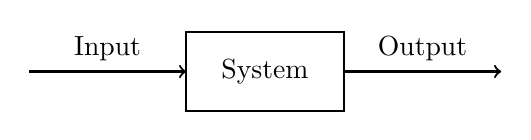
\begin{tikzpicture}
			\draw[thick, ->, color=black] (0,0) -- (2,0) node[midway, above] {Input};
			\draw[thick, color=black] (2,-0.5) rectangle (4,0.5) node[midway] {System};
			\draw[thick, ->, color=black] (4,0) -- (6,0) node[midway, above] {Output};
		\end{tikzpicture}
		\caption{Simple block diagram drawn with \texttt{tikz}.}
		\label{fig:tikz}
	\end{figure}
	
	%%%%%%%%%%%%%%%%%%%%%%%%%%%%%%%%%%%%%%%%%%%%%%%%%%%%%%%%%%%
	\subsection{\texttt{pgfplots}}
	The \texttt{pgfplots} package builds data plots on top of \texttt{tikz}. Plots go inside an \texttt{axis} environment, which handles the axis labels, tick marks, grid lines, and scaling for you. Use \texttt{\textbackslash addplot\{expression\}} to plot a mathematical function, or supply explicit coordinates to plot data points.
	
	Useful axis options include \texttt{width}, \texttt{height}, \texttt{xlabel}, \texttt{ylabel}, \texttt{xmin}/\texttt{xmax}, \texttt{ymin}/\texttt{ymax}, and \texttt{grid}. The \texttt{domain} option on \texttt{\textbackslash addplot} sets the range of $x$ values and \texttt{samples} controls how smooth the curve looks.
	
	\begin{figure}[H]
		\centering
		\begin{tikzpicture}
			\begin{axis}[
				width=0.75\linewidth,
				height=5cm,
				xlabel={$x$},
				ylabel={$y$},
				grid=major,
				grid style={color=themecolour!20},
				title={Title (Exclude this, figure caption acts as a title)},
				legend style={at={(1.02,0.5)}, anchor=west}]
				\addplot[color=themecolour, thick, domain=0:360, samples=100] {sin(x)};
				\addlegendentry{$\sin(x)$}
				\addplot[color=themecolour!50, thick, domain=0:360, samples=100] {cos(x)};
				\addlegendentry{$\cos(x)$}
			\end{axis}
		\end{tikzpicture}
		\caption{Sine and cosine waves plotted with \texttt{pgfplots}.}
		\label{fig:pgfplots}
	\end{figure}
	
	\begin{figure}[H]
		\centering
		\begin{tikzpicture}
			\begin{axis}[
				ybar,
				symbolic x coords={
					Category A,
					Category B,
					Category C,
					Category D
				},
				xtick=data,
				bar width=10pt,
				width=0.75\linewidth,
				height=5cm,
				nodes near coords,
				every node near coord/.append style={
					check for zero/.code={
						\pgfmathfloatifflags{\pgfplotspointmeta}{0}
						{\pgfkeys{/tikz/coordinate}}
						{}
					},
					check for zero
				},
				enlarge x limits=0.2,
				legend style={
					at={(1.02,0.5)},
					anchor=west
				},
				ymin=0,
				ymax=100,
				ylabel={Y‑Axis Label},
				xlabel={X‑Axis Label (Redundant here)},
				ymajorgrids=true,
				grid style={color=themecolour!20},
				]
				% Dataset 1
				\addplot[fill=themecolour!75] coordinates {
					(Category A,45)
					(Category B,70)
					(Category C,55)
					(Category D,25)
				};
				% Dataset 2
				\addplot[fill=themecolour!50] coordinates {
					(Category A,60)
					(Category B,40)
					(Category C,80)
					(Category D,50)
				};
				% Dataset 3
				\addplot[fill=themecolour!25] coordinates {
					(Category A,30)
					(Category B,35)
					(Category C,65)
					(Category D,75)
				};			
				\legend{Dataset 1, Dataset 2, Dataset 3}
			\end{axis}
		\end{tikzpicture}
		\caption{Bar graph plotted with \texttt{pgfplots}.}
		\label{fig:pgfbar}
	\end{figure}
	
	%%%%%%%%%%%%%%%%%%%%%%%%%%%%%%%%%%%%%%%%%%%%%%%%%%%%%%%%%%%
	\subsection{\texttt{circuitikz}}
	The \texttt{circuitikz} package extends \texttt{tikz} with circuit symbols for drawing electrical schematics. Components are placed along a path using \texttt{to[component, label]}, where the component name is a standard symbol such as \texttt{R} (resistor), \texttt{C} (capacitor), \texttt{L} (inductor), \texttt{V} (voltage source), or \texttt{I} (current source). Paths are chained together to form a closed loop.
	
	\begin{figure}[H]
		\centering
		\begin{circuitikz}
			\draw (0,0)
			to[V, l=$V_s$] (0,2)
			to[R, l=$R$]   (2,2)
			to[C, l=$C$]   (2,0)
			-- (0,0);
		\end{circuitikz}
		\caption{Simple RC circuit drawn with \texttt{circuitikz}.}
		\label{fig:circuit}
	\end{figure}
	
	%%%%%%%%%%%%%%%%%%%%%%%%%%%%%%%%%%%%%%%%%%%%%%%%%%%%%%%%%%%
	\subsection{\texttt{pgf-pie}}
	The \texttt{pgf-pie} package draws pie charts directly inside a \texttt{tikzpicture} environment. Each slice is specified as a percentage followed by a label, separated by a forward slash, and the values are listed inside the \texttt{\textbackslash pie} command. The package automatically scales the slices so that the percentages add up to a full circle.
	
	Useful options include \texttt{radius} to control the size of the chart, \texttt{text=legend} to place labels in a legend below instead of on the slices, \texttt{text=pin} to connect labels with lines, and \texttt{color} to supply a list of slice colours. Using \texttt{themecolour} with tints keeps the chart consistent with the rest of the document.
	
	\begin{figure}[H]
		\centering
		\begin{tikzpicture}
			\pie[
			color={themecolour!75, themecolour!50, themecolour!25, themecolour!0},
			radius=2.5,
			text=legend
			]{
				38/Product Development,
				27/Marketing \& Sales,
				20/Operations,
				15/Research \& Development
			}
		\end{tikzpicture}
		\caption{Annual budget allocation across departments.}
		\label{fig:pie-budget}
	\end{figure}
	
	%%%%%%%%%%%%%%%%%%%%%%%%%%%%%%%%%%%%%%%%%%%%%%%%%%%%%%%%%%%
	\subsection{\texttt{environ}}
	\noindent\colorbox{themecolour!15}{\parbox{\linewidth}{\small This package is used internally by the template for draft-mode figure suppression. Users do not use it directly.}}\vspace{0.5\baselineskip}
	
	The \texttt{environ} package lets the template capture the contents of a \texttt{tikzpicture} or \texttt{circuitikz} environment without running them. When \texttt{\textbackslash metaShowFigures} is \texttt{false}, this is what allows vector graphics to be replaced with a lightweight placeholder box instead of being fully computed and drawn, which speeds up compiling while drafting.

%%%%%%%%%%%%%%%%%%%%%%%%%%%%%%%%%%%%%%%%%%%%%%%%%%%%%%%%%%%
% ALGORITHMS
%%%%%%%%%%%%%%%%%%%%%%%%%%%%%%%%%%%%%%%%%%%%%%%%%%%%%%%%%%%
\section{Algorithms}

	%%%%%%%%%%%%%%%%%%%%%%%%%%%%%%%%%%%%%%%%%%%%%%%%%%%%%%%%%%%
	\subsection{\texttt{algorithm} and \texttt{algpseudocode}}
	The \texttt{algorithm} package provides a float wrapper for pseudocode, giving algorithms captions, labels, and an entry in a list of algorithms, the same way \texttt{figure} wraps a \texttt{tikzpicture}. The \texttt{algpseudocode} package supplies the pseudocode commands that go inside the \texttt{algorithmic} environment.
	
	The \texttt{algorithmic} environment takes an optional line-numbering argument: \texttt{[1]} numbers every line, \texttt{[2]} numbers every second line, and omitting it disables numbering entirely.
	
	\begin{tabularx}{\linewidth}{@{}lL@{}}
		\caption{Common \texttt{algpseudocode} commands.}
		\label{tab:algpseudocode} \\
		\toprule
		%%%%% HEADER ROW(S) %%%%%
		Command & Purpose \\
		\midrule
		\endfirsthead
		\toprule
		%%%%% HEADER ROW(S) %%%%%
		Command & Purpose \\
		\midrule
		\endhead
		\bottomrule
		\endfoot
		\bottomrule
		%%%%% NOTES %%%%%
		% NOTES HERE
		\endlastfoot
		%%%%% START %%%%%
		\texttt{\textbackslash Require} & Declares what the algorithm expects as input \\
		
		\texttt{\textbackslash Ensure}  & Declares what the algorithm produces as output \\
		
		\texttt{\textbackslash State}   & A single statement on its own line \\
		
		\texttt{\textbackslash Function\{name\}\{params\}} & Opens a named function block \\
		
		\texttt{\textbackslash If / \textbackslash ElsIf / \textbackslash Else / \textbackslash EndIf} & Conditional branch \\
		
		\texttt{\textbackslash For / \textbackslash EndFor} & For loop \\
		
		\texttt{\textbackslash While / \textbackslash EndWhile} & While loop \\
		
		\texttt{\textbackslash Return} & Return statement \\
		
		\texttt{\textbackslash Comment\{...\}} & Inline comment, right-aligned \\
	\end{tabularx}
	
	The two algorithms below demonstrate a function with nested control flow. Indentation is handled automatically with no manual spacing required:
	
	\begin{algorithm}[H]
		\caption{Binary Search}
		\label{alg:binarysearch}
		\begin{algorithmic}[1]
			\Require Sorted array $A$ of length $n$, search value $target$
			\Ensure Index of $target$ in $A$, or $-1$ if not found
			\Function{BinarySearch}{$A, n, target$}
			\State $low \gets 0$
			\State $high \gets n - 1$
			\While{$low \leq high$}
			\State $mid \gets \lfloor(low + high) / 2\rfloor$ \Comment{Compute midpoint}
			\If{$A[mid] = target$}
			\State \Return $mid$ \Comment{Target found}
			\ElsIf{$A[mid] < target$}
			\State $low \gets mid + 1$ \Comment{Search right half}
			\Else
			\State $high \gets mid - 1$ \Comment{Search left half}
			\EndIf
			\EndWhile
			\State \Return $-1$ \Comment{Target not found}
			\EndFunction
		\end{algorithmic}
	\end{algorithm}
	
	\begin{algorithm}[H]
		\caption{Bubble Sort}
		\label{alg:bubblesort}
		\begin{algorithmic}[1]
			\Require Array $A$ of length $n$
			\Ensure $A$ sorted in ascending order
			\Function{BubbleSort}{$A, n$}
			\For{$i \gets 0$ \textbf{to} $n - 1$}
			\For{$j \gets 0$ \textbf{to} $n - i - 2$}
			\If{$A[j] > A[j+1]$}
			\State swap $A[j]$ and $A[j+1]$ \Comment{Swap out-of-order elements}
			\EndIf
			\EndFor
			\EndFor
			\EndFunction
		\end{algorithmic}
	\end{algorithm}
	
	Algorithms are referenced using \texttt{\textbackslash cref} like any other float. \cref{alg:binarysearch} searches a sorted list by repeatedly halving the search range, while \cref{alg:bubblesort} sorts a list by repeatedly swapping neighbouring elements that are in the wrong order.

%%%%%%%%%%%%%%%%%%%%%%%%%%%%%%%%%%%%%%%%%%%%%%%%%%%%%%%%%%%
% LINKS & REFERENCES
%%%%%%%%%%%%%%%%%%%%%%%%%%%%%%%%%%%%%%%%%%%%%%%%%%%%%%%%%%%
\section{Links \& References}

	%%%%%%%%%%%%%%%%%%%%%%%%%%%%%%%%%%%%%%%%%%%%%%%%%%%%%%%%%%%
	\subsection{\texttt{hyperref}}
	\noindent\colorbox{themecolour!15}{\parbox{\linewidth}{\small This package is used internally by the template to configure clickable links and PDF metadata. Users interact with it through \texttt{\textbackslash url\{\}} and \texttt{\textbackslash href\{\}\{\}} for external links; all internal cross-references are handled automatically.}}\vspace{0.5\baselineskip}
	
	The \texttt{hyperref} package makes every internal cross-reference, citation, and table of contents entry clickable in the PDF. It also embeds document information such as the title and author into the PDF file. The template sets all link colours to \texttt{themecolour} automatically.
	
	The two commands you will use directly are \texttt{\textbackslash url\{\}} for a plain clickable link and \texttt{\textbackslash href\{url\}\{text\}} for a link with custom display text:
	
	\begin{itemize}[noitemsep]
		\item \texttt{\textbackslash url\{https://www.yorku.ca\}} $\to$ \url{https://www.yorku.ca}
		\item \texttt{\textbackslash href\{https://www.yorku.ca\}\{York University\}} $\to$ \href{https://www.yorku.ca}{York University}
	\end{itemize}
	
	%%%%%%%%%%%%%%%%%%%%%%%%%%%%%%%%%%%%%%%%%%%%%%%%%%%%%%%%%%%
	\subsection{\texttt{cleveref}}
	\noindent\colorbox{themecolour!15}{\parbox{\linewidth}{\small This package is used internally by the template to configure reference formatting. Users interact with it directly through \texttt{\textbackslash cref\{\}} and \texttt{\textbackslash Cref\{\}} for all cross-references.}}\vspace{0.5\baselineskip}
	
	The \texttt{cleveref} package replaces the standard \texttt{\textbackslash ref} command with \texttt{\textbackslash cref}, which automatically adds the correct label type in front of the number. For example, \texttt{\textbackslash cref\{fig:logo\}} produces \cref{fig:logo} without you having to type the word ``Figure'' yourself. Use \texttt{\textbackslash Cref} (capital C) at the start of a sentence. You can also pass multiple labels separated by commas and \texttt{cleveref} will group them neatly.
	
	\begin{tabularx}{\linewidth}{@{}ll@{}}
		\caption{Cross-reference examples using \texttt{\textbackslash cref} for lowercase and \texttt{\textbackslash Cref} for uppercase.}
		\label{tab:cleveref} \\
		\toprule
		%%%%% HEADER ROW(S) %%%%%
		Type & Output \\
		\midrule
		\endfirsthead
		\toprule
		%%%%% HEADER ROW(S) %%%%%
		Type & Output \\
		\midrule
		\endhead
		\bottomrule
		\endfoot
		\bottomrule
		%%%%% NOTES %%%%%
		% NOTES HERE
		\endlastfoot
		%%%%% START %%%%%
		\multicolumn{2}{c}{\texttt{\textbackslash cref}} \\
		Figure      & \cref{fig:logo} \\
		Sub-figure  & \cref{fig:sub_a} \\
		Table       & \cref{tab:booktabs} \\
		Equation    & \cref{eq:simple} \\
		Reaction    & \cref{rxn:combustion} \\
		Algorithm   & \cref{alg:binarysearch} \\
		Section     & \cref{sec:lists} \\
		Appendix	& \cref{sec:appendix-supp} \\
		Theorem     & \cref{thm:pythagorean} \\
		Lemma       & \cref{lem:even} \\
		Proposition & \cref{prop:rational} \\
		Corollary   & \cref{cor:prime} \\
		Conjecture  & \cref{con:goldbach} \\
		Axiom       & \cref{axm:line} \\
		Definition  & \cref{def:even} \\
		Example     & \cref{ex:even} \\
		Criterion   & \cref{crit:positive} \\
		Remark      & \cref{rem:zero} \\
		Note        & \cref{note:numbering} \\
		Problem     & \cref{prob:ohmslaw} \\
		Listing     & \cref{lst:MATLAB} \\
		\midrule
		\multicolumn{2}{c}{\texttt{\textbackslash Cref}} \\
		Figure      & \Cref{fig:logo} \\
		Sub-figure  & \Cref{fig:sub_a} \\
		Table       & \Cref{tab:booktabs} \\
		Equation    & \Cref{eq:simple} \\
		Reaction    & \Cref{rxn:combustion} \\
		\multicolumn{2}{c}{\textit{etc...}} \\
	\end{tabularx}

%%%%%%%%%%%%%%%%%%%%%%%%%%%%%%%%%%%%%%%%%%%%%%%%%%%%%%%%%%%
% TYPOGRAPHY
%%%%%%%%%%%%%%%%%%%%%%%%%%%%%%%%%%%%%%%%%%%%%%%%%%%%%%%%%%%
\section{Typography}

	%%%%%%%%%%%%%%%%%%%%%%%%%%%%%%%%%%%%%%%%%%%%%%%%%%%%%%%%%%%
	\subsection{\texttt{microtype}}
	\noindent\colorbox{themecolour!15}{\parbox{\linewidth}{\small This package is used internally by the template to improve text rendering. It requires no user configuration and produces no visually distinct output on its own.}}\vspace{0.5\baselineskip}
	
	The \texttt{microtype} package makes small automatic adjustments to character spacing and sizing to produce cleaner, more even-looking paragraphs. The result is fewer lines that stick out into the margin and less awkward hyphenation, particularly in dense paragraphs with long words. It works silently in the background with no action needed from you.
	
	%%%%%%%%%%%%%%%%%%%%%%%%%%%%%%%%%%%%%%%%%%%%%%%%%%%%%%%%%%%
	\subsection{\texttt{xurl}}
	\noindent\colorbox{themecolour!15}{\parbox{\linewidth}{\small This package is used internally by the template to improve URL line breaking. Users interact with it through \texttt{\textbackslash url\{\}}, which is provided by \texttt{hyperref}.}}\vspace{0.5\baselineskip}
	
	The \texttt{xurl} package allows long URLs to break across lines at sensible points such as slashes, dots, and hyphens. Without it, a long URL is treated as one unbreakable word and can stick out past the margin. The URL below is long enough to demonstrate a clean line break:
	
	\url{https://futurestudents.yorku.ca/program/engineering-intl-development-studies}
	
	%%%%%%%%%%%%%%%%%%%%%%%%%%%%%%%%%%%%%%%%%%%%%%%%%%%%%%%%%%%
	\subsection{\texttt{indentfirst}}
	\noindent\colorbox{themecolour!15}{\parbox{\linewidth}{\small This package is used internally by the template to enforce consistent paragraph indentation. It requires no user configuration.}}\vspace{0.5\baselineskip}
	
	By default, \LaTeX{} does not indent the first paragraph of a section. The \texttt{indentfirst} package changes this so every paragraph is indented, including the first one. The paragraph below is the first in this subsection and is indented because \texttt{indentfirst} is loaded:
	
	This is the first paragraph of this subsection, it is indented because \texttt{indentfirst} is loaded.
	
	This is the second paragraph, also indented as normal.
	
	%%%%%%%%%%%%%%%%%%%%%%%%%%%%%%%%%%%%%%%%%%%%%%%%%%%%%%%%%%%
	\subsection{\texttt{ragged2e}}
	\noindent\colorbox{themecolour!15}{\parbox{\linewidth}{\small This package is used internally by the template to improve text alignment in captions, boxes, and tables. Users interact with it through the column types \texttt{L}, \texttt{C}, \texttt{R}, \texttt{P\{\}}, \texttt{Q\{\}}, and \texttt{S\{\}} defined in the template.}}\vspace{0.5\baselineskip}
	
	The \texttt{ragged2e} package provides improved versions of \LaTeX{}'s built-in alignment commands. The standard \texttt{\textbackslash raggedright}, \texttt{\textbackslash centering}, and \texttt{\textbackslash raggedleft} commands disable hyphenation entirely, which can produce very uneven line lengths. The \texttt{ragged2e} versions (\texttt{\textbackslash RaggedRight}, \texttt{\textbackslash Centering}, and \texttt{\textbackslash RaggedLeft}) allow hyphenation while still keeping text ragged, resulting in much more even-looking paragraphs. The template applies these automatically to captions, problem and solution boxes, and the custom table column types.

%%%%%%%%%%%%%%%%%%%%%%%%%%%%%%%%%%%%%%%%%%%%%%%%%%%%%%%%%%%
% LISTS
%%%%%%%%%%%%%%%%%%%%%%%%%%%%%%%%%%%%%%%%%%%%%%%%%%%%%%%%%%%
\section{Lists}\label{sec:lists}

	%%%%%%%%%%%%%%%%%%%%%%%%%%%%%%%%%%%%%%%%%%%%%%%%%%%%%%%%%%%
	\subsection{\texttt{enumitem}}
	The \texttt{enumitem} package gives you extra control over the spacing, labels, and indentation of \LaTeX's three built-in list environments: \texttt{itemize}, \texttt{enumerate}, and \texttt{description}. Options are passed in square brackets directly on the environment.
	
	The most useful option is \texttt{noitemsep}, which removes the extra vertical gap that \LaTeX{} normally adds between items. Use it when list items are short and you want a tighter look:
	
	\begin{itemize}[noitemsep]
		\item First item
		\item Second item
		\item Third item
	\end{itemize}
	
	The \texttt{label} option lets you change the bullet or number style. Use \texttt{\textbackslash arabic*} for numbers, \texttt{\textbackslash alph*} for lowercase letters, \texttt{\textbackslash Alph*} for uppercase letters, \texttt{\textbackslash roman*} for lowercase roman numerals, and \texttt{\textbackslash Roman*} for uppercase roman numerals. The \texttt{*} is replaced by the item number automatically:
	
	\begin{enumerate}[label=\textbf{\arabic*.}, noitemsep]
		\item First item
		\item Second item
		\item Third item
	\end{enumerate}
	
	\begin{enumerate}[label=(\alph*), noitemsep]
		\item First item
		\item Second item
		\item Third item
	\end{enumerate}
	
	The \texttt{description} environment is useful for glossaries and key-value lists where each item has a bold label followed by a short explanation. The \texttt{leftmargin} option controls how far the body text is indented, and \texttt{style=nextline} places the body on a new line below the label, which helps when labels are long:
	
	\begin{description}[leftmargin=3cm, style=nextline]
		\item[\texttt{noitemsep}] Removes vertical space between items and between the list and surrounding text
		\item[\texttt{label}] Overrides the default bullet or numbering style with any arbitrary format
		\item[\texttt{leftmargin}] Controls the left indent of the list body relative to the page margin
		\item[\texttt{style=nextline}] Places the description body on a new line below the label
	\end{description}
	
	Lists can be nested up to three levels deep. Indentation and bullet styles adjust automatically at each level:
	
	\begin{itemize}
		\item First level item
		\begin{itemize}[noitemsep]
			\item Second level item
			\begin{itemize}[noitemsep]
				\item Third level item
			\end{itemize}
		\end{itemize}
		\item Another first level item
	\end{itemize}

%%%%%%%%%%%%%%%%%%%%%%%%%%%%%%%%%%%%%%%%%%%%%%%%%%%%%%%%%%%
% PROBLEM / SOLUTION ENVIRONMENTS
%%%%%%%%%%%%%%%%%%%%%%%%%%%%%%%%%%%%%%%%%%%%%%%%%%%%%%%%%%%
\section{Problem \& Solution Environments}

	%%%%%%%%%%%%%%%%%%%%%%%%%%%%%%%%%%%%%%%%%%%%%%%%%%%%%%%%%%%
	\subsection{\texttt{tcolorbox}}
	\noindent\colorbox{themecolour!15}{\parbox{\linewidth}{\small This package is used internally by the template to define the \texttt{problem} and \texttt{solution} environments. Users interact with it through those environments directly; the underlying \texttt{tcolorbox} configuration requires no modification.}}\vspace{0.5\baselineskip}
	
	The \texttt{tcolorbox} package provides the \texttt{problem} and \texttt{solution} environments. The \texttt{problem} environment is numbered automatically. When \texttt{\textbackslash metaNumberProblems} is set to \texttt{true} in \texttt{main.tex}, problems are numbered by section (e.g.\ Problem 2.1, Problem 2.2). When set to \texttt{false}, problems are numbered from 1 continuously through the whole document. An optional title can be added in square brackets after \texttt{\textbackslash begin\{problem\}} and it will appear in the header bar next to the number.
	
	\begin{problem}[Ohm's Law]
		\label{prob:ohmslaw}
		Given a resistor $R = \SI{10}{\ohm}$ with a voltage $V = \SI{5}{\volt}$ across it,
		find the current $I$.
	\end{problem}
	
	\begin{solution}
		Applying Ohm's Law:
		\begin{equation}
			I = \frac{V}{R} = \frac{5}{10} = \SI{0.5}{\ampere}
		\end{equation}
		\qed
	\end{solution}
	
	The title argument is optional. When omitted, only the problem number appears in the header:
	
	\begin{problem}
		\label{prob:problem}
		A problem without a title is also valid.
	\end{problem}

%%%%%%%%%%%%%%%%%%%%%%%%%%%%%%%%%%%%%%%%%%%%%%%%%%%%%%%%%%%
% CODE LISTINGS
%%%%%%%%%%%%%%%%%%%%%%%%%%%%%%%%%%%%%%%%%%%%%%%%%%%%%%%%%%%
\section{Code Listings}

Every code block in this template, whether highlighted by \texttt{listings} or \texttt{minted}, is captioned and numbered off the same \texttt{lstlisting} counter. Place a \texttt{\textbackslash captionof\{lstlisting\}\{...\}} and \texttt{\textbackslash label\{...\}} directly above the code, and reference it anywhere with \texttt{\textbackslash cref}/\texttt{\textbackslash Cref} as usual. Because both engines write to the same counter, listings and minted blocks number continuously through one shared sequence no matter which produced a given block.

	%%%%%%%%%%%%%%%%%%%%%%%%%%%%%%%%%%%%%%%%%%%%%%%%%%%%%%%%%%%
	\subsection{\texttt{listings}}
	\noindent\colorbox{themecolour!15}{\parbox{\linewidth}{\small \texttt{listings} is a drafting-speed fallback: it is what powers the \texttt{codelisting} environment whenever \texttt{\textbackslash metaUseMinted} is \texttt{false}. Since it compiles natively (no external calls), it is fast, but its highlighting is less accurate and covers fewer languages than \texttt{minted}. Keep it on while drafting, and switch to \texttt{minted} for a final compile.}}\vspace{0.5\baselineskip}
	
	The \texttt{listings} package displays source code with syntax highlighting and line numbers. Five named styles are built into this template: \texttt{matlab}, \texttt{java}, \texttt{python}, \texttt{cpp}, and \texttt{latex}. All styles share the same base look: a monospaced font, line numbers on the left in \texttt{themecolour}, a light grey background, and automatic line wrapping. Select a style by adding \texttt{style=name} as an option on the \texttt{lstlisting} environment.
	
	For short inline code snippets, use \texttt{\textbackslash lstinline[style=name]|...|} with \texttt{|} as the delimiter on both sides.
	
	%%%%%%%%%%%%%%%%%%%%%%%%%%%%%%%%%%%%%%%%%%%%%%%%%%%%%%%%%%%
	\subsection{\texttt{minted}}\label{sec:minted}
	\noindent\colorbox{themecolour!15}{\parbox{\linewidth}{\small This package is optional and controlled by \texttt{\textbackslash metaUseMinted} in \texttt{main.tex}. It requires the \texttt{-8bit -shell-escape} compiler flag and a working Python/Pygments install.}}\vspace{0.5\baselineskip}
	
	\texttt{minted} is the \textbf{preferred} engine for code listings in this template, used automatically by the \texttt{codelisting} environment whenever \texttt{\textbackslash metaUseMinted} is \texttt{true}. It uses the Python library Pygments to perform syntax highlighting instead of \LaTeX{} macros, producing more accurate, professional-looking highlighting for a much wider range of languages than \texttt{listings} can match.
	
	This accuracy comes at a real cost: \texttt{minted} shells out to Pygments on every compile, which is noticeably \textbf{slower} than \texttt{listings}' native, in-\TeX{} highlighting. For that reason, it is recommended to leave \texttt{\textbackslash metaUseMinted} set to \texttt{false} while actively drafting, and only switch it to \texttt{true} for a final, polished compile.
	
	\ifmetaUseMinted
	
	To use \texttt{minted}, compile with the \texttt{-8bit -shell-escape} flag enabled, and ensure Python and Pygments are installed and available on your system's PATH.
	
	Use \texttt{\textbackslash mintinline\{language\}\{code\}} for a short inline snippet:
	
	\mintinline{java}{public class HelloWorld {}
	}
	
	Unlike \texttt{\textbackslash lstinline}, the block form of \texttt{minted} cannot be placed inside a table cell or a \texttt{tcolorbox} (including this template's \texttt{problem} and \texttt{solution} environments), since both rely on verbatim reading that conflicts with those contexts. Use \texttt{\textbackslash mintinline\{\}\{\}} in those situations instead.
	
	\else
	
	\texttt{minted} is currently \textbf{disabled}. Set \texttt{\textbackslash metaUseMinted\{true\}} in \texttt{main.tex} and compile with the \texttt{-8bit -shell-escape} flag to enable Pygments-based syntax highlighting and see a live demo here.
	
	\fi
	
	%%%%%%%%%%%%%%%%%%%%%%%%%%%%%%%%%%%%%%%%%%%%%%%%%%%%%%%%%%%
	\subsection{\texttt{codelisting} Environments}
	\noindent\colorbox{themecolour!15}{\parbox{\linewidth}{\small \texttt{codelisting} is this template's unified code environment. It automatically renders using \texttt{minted} or \texttt{listings}, whichever is currently active per \texttt{\textbackslash metaUseMinted}, so every code block in a document uses one consistent syntax regardless of which engine produces it.}}\vspace{0.5\baselineskip}
	
	Write \texttt{\textbackslash begin\{codelisting\}\{style\}...\textbackslash end\{codelisting\}}, where \texttt{style} matches one of the named styles defined in \texttt{stemtemplate.sty} (\texttt{matlab}, \texttt{java}, \texttt{python}, \texttt{cpp}, \texttt{latex}). The same style name is used whether \texttt{minted} is on or off.
	
		%%%%%%%%%%%%%%%%%%%%%%%%%%%%%%%%%%%%%%%%%%%%%%%%%%%%%%%%%%%
		\subsubsection{MATLAB}
{\vspace{10pt}
	\captionof{lstlisting}{MATLAB example.}
	\label{lst:MATLAB}
	\vspace{-4pt}}
\begin{codelisting}{matlab}
	x = 0:0.1:2*pi; % This is a comment
	y = sin(x);
	plot(x, y);
	xlabel('x'); ylabel('sin(x)');
	title('Sine Wave');
\end{codelisting}
		
		%%%%%%%%%%%%%%%%%%%%%%%%%%%%%%%%%%%%%%%%%%%%%%%%%%%%%%%%%%%
		\subsubsection{Java}
{\vspace{10pt}
	\captionof{lstlisting}{Java example.}
	\label{lst:java}
	\vspace{-4pt}}
\begin{codelisting}{java}
	public class HelloWorld {
		public static void main(String[] args) {
			System.out.println("Hello, World!");
		} // This is a comment
	}
\end{codelisting}
		
		%%%%%%%%%%%%%%%%%%%%%%%%%%%%%%%%%%%%%%%%%%%%%%%%%%%%%%%%%%%
		\subsubsection{Python}
{\vspace{10pt}
	\captionof{lstlisting}{Python example.}
	\label{lst:python}
	\vspace{-4pt}}
\begin{codelisting}{python}
	import numpy as np
	import matplotlib.pyplot as plt
	
	x = np.linspace(0, 2 * np.pi, 100)
	y = np.sin(x)
	plt.plot(x, y)
	plt.show()
\end{codelisting}
		
		%%%%%%%%%%%%%%%%%%%%%%%%%%%%%%%%%%%%%%%%%%%%%%%%%%%%%%%%%%%
		\subsubsection{C++}
{\vspace{10pt}
	\captionof{lstlisting}{C++ example.}
	\label{lst:cpp}
	\vspace{-4pt}}
\begin{codelisting}{cpp}
	#include <iostream>
	using namespace std;
	
	int main() {
		cout << "Hello, World!" << endl;
		return 0;
	}
\end{codelisting}
		
		%%%%%%%%%%%%%%%%%%%%%%%%%%%%%%%%%%%%%%%%%%%%%%%%%%%%%%%%%%%
		\subsubsection{LaTeX}
{\vspace{10pt}
	\captionof{lstlisting}{LaTeX example.}
	\label{lst:latex}
	\vspace{-4pt}}
\begin{codelisting}{latex}
	\begin{equation} % This is a comment
		E = mc^2
		\label{eq:einstein}
	\end{equation}
	See \cref{eq:einstein} for Einstein's mass-energy equivalence.
\end{codelisting}

%%%%%%%%%%%%%%%%%%%%%%%%%%%%%%%%%%%%%%%%%%%%%%%%%%%%%%%%%%%
% HEADER & FOOTER
%%%%%%%%%%%%%%%%%%%%%%%%%%%%%%%%%%%%%%%%%%%%%%%%%%%%%%%%%%%
\section{Header \& Footer}

	%%%%%%%%%%%%%%%%%%%%%%%%%%%%%%%%%%%%%%%%%%%%%%%%%%%%%%%%%%%
	\subsection{\texttt{fancyhdr}}
	\noindent\colorbox{themecolour!15}{\parbox{\linewidth}{\small This package is used internally by the template to configure the page header and footer. Users control the content through metadata fields in \texttt{main.tex}; the \texttt{fancyhdr} configuration itself requires no modification.}}\vspace{0.5\baselineskip}
	
	The \texttt{fancyhdr} package gives you full control over the header and footer on every page. It divides both the header and footer into three zones: left, centre, and right. Each zone is set with its own command: \texttt{\textbackslash lhead}, \texttt{\textbackslash chead}, and \texttt{\textbackslash rhead} for the header, and \texttt{\textbackslash lfoot}, \texttt{\textbackslash cfoot}, and \texttt{\textbackslash rfoot} for the footer. The template fills these zones automatically using your metadata, so you do not need to call any of these commands yourself.
	
	The decorative rule below the header is coloured in \texttt{themecolour} and its thickness is set to \texttt{0.8pt} by the template. You can also define different headers for different sections of the document or for odd and even pages if needed.
	
		%%%%%%%%%%%%%%%%%%%%%%%%%%%%%%%%%%%%%%%%%%%%%%%%%%%%%%%%%%%
		\subsubsection{Smart Collision Logic}
		The template includes a custom \texttt{\textbackslash smartleftheader} command that automatically adjusts the left side of the header to prevent it from overlapping with the right side. It does this by measuring the available horizontal space and choosing one of four display modes:
		
		\begin{enumerate}[noitemsep]
			\item \textbf{Full Mode}: Shows the course code followed by the full course name.
			\item \textbf{Acronym Mode}: If the full name is too long, it is shortened to an acronym (e.g., ``Object-Oriented Programming \& Telemetry'' becomes ``OOP\&T'').
			\item \textbf{Minimal Mode}: If even the acronym is too long, only the course code is shown.
			\item \textbf{Hidden Mode}: If the right side takes up nearly the full width, the left header is hidden completely to keep the header readable.
		\end{enumerate}
		
		\begin{tabularx}{\linewidth}{@{}ll@{}}
			\caption{Dynamic header states based on available width.}
			\label{tab:header_logic} \\
			\toprule
			%%%%% HEADER ROW(S) %%%%%
			Scenario & Left Header Output \\
			\midrule
			\endfirsthead
			\toprule
			%%%%% HEADER ROW(S) %%%%%
			Scenario & Left Header Output \\
			\midrule
			\endhead
			\bottomrule
			\endfoot
			\bottomrule
			%%%%% NOTES %%%%%
			% NOTES HERE
			\endlastfoot
			%%%%% START %%%%%
			Not Crowded   & \metaCourseCode: \metaCourseName \\
			
			A Little Crowded & \metaCourseCode: \makeAcronym{\metaCourseName} \\
			
			Crowded       & \metaCourseCode \\
			
			Overcrowded   & (Hidden) \\
		\end{tabularx}
		
		The acronym is generated by the \texttt{\textbackslash makeAcronym} command, which takes the first letter of each significant word in \texttt{\textbackslash metaCourseName} and skips short words like ``the'', ``of'', and ``to''. See \cref{tab:xstring} for the string commands it uses internally.

%%%%%%%%%%%%%%%%%%%%%%%%%%%%%%%%%%%%%%%%%%%%%%%%%%%%%%%%%%%
% BIBLIOGRAPHY
%%%%%%%%%%%%%%%%%%%%%%%%%%%%%%%%%%%%%%%%%%%%%%%%%%%%%%%%%%%
\section{Bibliography}

	%%%%%%%%%%%%%%%%%%%%%%%%%%%%%%%%%%%%%%%%%%%%%%%%%%%%%%%%%%%
	\subsection{\texttt{csquotes}}
	\noindent\colorbox{themecolour!15}{\parbox{\linewidth}{\small This package is used internally by the template and is required by \texttt{biblatex}. It produces no visible output and requires no user configuration.}}\vspace{0.5\baselineskip}
	
	The \texttt{csquotes} package is a behind-the-scenes dependency of \texttt{biblatex} that ensures quotation marks in bibliography entries are typeset correctly for the active language. You can also use it directly in your document with \texttt{\textbackslash enquote\{\}} to wrap a phrase in the correct quotation marks for English: \enquote{This is a quoted phrase.}
	
	%%%%%%%%%%%%%%%%%%%%%%%%%%%%%%%%%%%%%%%%%%%%%%%%%%%%%%%%%%%
	\subsection{\texttt{biblatex}}\label{sec:biblatex}
	The \texttt{biblatex} package handles all citation formatting and bibliography generation. References are stored in a \texttt{.bib} file, cited in the document with \texttt{\textbackslash autocite\{key\}} (or one of several style-specific variants), and the full bibliography is printed at the end with \texttt{\textbackslash printbibliography}.
	
	\Cref{tab:biblatexcommands} summarizes the available citation commands, and \cref{tab:biblatexstyles} lists the supported citation styles. The active style is set via \texttt{\textbackslash metaBibStyle} in \texttt{main.tex}; the style currently active in this document is \texttt{\metaBibStyle}.
	
	\begin{tabularx}{\linewidth}{@{}lcL@{}}
		\caption{Standard \texttt{biblatex} citation commands and descriptions.}
		\label{tab:biblatexcommands} \\
		\toprule
		%%%%% HEADER ROW(S) %%%%%
		Command & Output Format & Description \\
		\midrule
		\endfirsthead
		\toprule
		%%%%% HEADER ROW(S) %%%%%
		Command & Output Format & Description \\
		\midrule
		\endhead
		\bottomrule
		\endfoot
		\bottomrule
		%%%%% NOTES %%%%%
		% NOTES HERE
		\endlastfoot
		%%%%% START %%%%%
		\texttt{\textbackslash autocite\{key\}}     & High-level context   & \textbf{Recommended default.} Automatically adapts to the active style (parenthetical, superscript, or footnote). \\
		\addlinespace
		
		\texttt{\textbackslash cite\{key\}}         & Bare citation         & Basic citation output without extra surrounding parentheses or brackets (unless defined by style). \\
		\addlinespace
		
		\texttt{\textbackslash parencite\{key\}}    & Parenthetical         & Encloses the citation in brackets or parentheses, e.g., \texttt{[1]} or \texttt{(Smith, 2026)}. \\
		\addlinespace
		
		\texttt{\textbackslash textcite\{key\}}     & Narrative / In-text   & Integrates author name into sentence prose, e.g., \texttt{Smith [1]} or \texttt{Smith (2026)}. \\
		\addlinespace
		
		\texttt{\textbackslash supercite\{key\}}    & Superscript           & Forces citation as a superscript number, e.g., \textsuperscript{1} or \textsuperscript{1,2}. \\
		\addlinespace
		
		\texttt{\textbackslash footcite\{key\}}     & Footnote              & Places full or abbreviated citation in a footnote at the bottom of the page. \\
		\addlinespace
		
		\texttt{\textbackslash citeauthor\{key\}}   & Author name(s) only   & Prints only author names without year or index, e.g., \texttt{Smith et al.} \\
		\addlinespace
		
		\texttt{\textbackslash citeyear\{key\}}     & Publication year only & Prints only the publication year, e.g., \texttt{2026}. \\
		\addlinespace
		
		\texttt{\textbackslash citetitle\{key\}}    & Title string only     & Prints only the title of the entry, e.g., \texttt{Thermal Control Design}. \\
		\addlinespace
		
		\texttt{\textbackslash citeurl\{key\}}      & URL link              & Extracts and prints only the URL field from the entry. \\
		\addlinespace
		
		\texttt{\textbackslash nocite\{key\}}       & Invisible             & Includes the entry in the final bibliography without generating in-text output. Pass \texttt{*} to print all items. \\
		
		\midrule
		
		\texttt{\textbackslash cite[2]\{key\}} 		& Page 					& Passes a specific page or section number, e.g., \texttt{[1, p. 2]} or \texttt{(Smith, 2026, p. 2)}. \\
		\addlinespace
		
		\texttt{\textbackslash cite[2-3]\{key\}} 	& Pages 				& Passes a specific page or section number, e.g., \texttt{[1, pp. 2-3]} or \texttt{(Smith, 2026, pp. 2-3)}. \\
		\addlinespace
		
		\texttt{[\textbackslash bibstring\{paragraph\}~4]} & Paragraph & Suppresses default \texttt{p.} and inserts \texttt{par.}, e.g., \texttt{[1, par. 4]}. \\
	\end{tabularx}
	
	\begin{tabularx}{\linewidth}{@{}lccc@{}}
		\caption{BibLaTeX citation styles.}
		\label{tab:biblatexstyles} \\
		\toprule
		%%%%% HEADER ROW(S) %%%%%
		Input & Name & Field & Example Output \\
		\midrule
		\endfirsthead
		\toprule
		%%%%% HEADER ROW(S) %%%%%
		Input & Name & Field & Example Output \\
		\midrule
		\endhead
		\bottomrule
		\endfoot
		\bottomrule
		%%%%% NOTES %%%%%
		% NOTES HERE
		\endlastfoot
		%%%%% START %%%%%
		\texttt{chem-acs}           & ACS     & Chemistry             & \textsuperscript{1} \\
		
		\texttt{phys}               & AIP     & Physics / Astronomy   & \textsuperscript{1} \\
		
		\texttt{nature}             & Nature  & Multidisciplinary Sci.& \textsuperscript{1} \\
		
		\texttt{science}            & Science & Multidisciplinary Sci.& \texttt{(1)} \\
		
		\texttt{ieee}               & IEEE    & Engineering           & \texttt{[1]} or \texttt{[1-3]} \\
		
		\texttt{mla}                & MLA     & Literature / Arts     & \texttt{(Smith 42)} \\
		
		\texttt{apa}                & APA     & Psychology / Education & \texttt{(Smith, 2026)} \\
	\end{tabularx}
	
	After adding new references to the \texttt{.bib} file, Biber must be run once between compilations for new citations to resolve. Most editors, such as Overleaf and TeXstudio, handle this automatically when configured to use Biber as the bibliography backend.
	
	For example, \texttt{\textbackslash autocite[1-2]\{example\}} produces: \autocite[1-2]{example}

% REFERENCES ----------------------------------------------
\clearpage
\phantomsection % Allows TOC to link to references
\printbibliography[heading=bibintoc] % Need square bracket content for TOC

%%%%%%%%%%%%%%%%%%%%%%%%%%%%%%%%%%%%%%%%%%%%%%%%%%%%%%%%%%%
% APPENDICES
%%%%%%%%%%%%%%%%%%%%%%%%%%%%%%%%%%%%%%%%%%%%%%%%%%%%%%%%%%%
\appendix % Insert this to create appendix

% APPENDIX A ----------------------------------------------
%%%%%%%%%%%%%%%%%%%%%%%%%%%%%%%%%%%%%%%%%%%%%%%%%%%%%%%%%%%
\clearpage
\section{Appendices}\label{sec:appendix-supp}

Place appendices at the end of your document after the bibliography. The \texttt{\textbackslash appendix} command switches section numbering from arabic numbers to uppercase letters, so each \texttt{\textbackslash section\{\}} after it becomes a new appendix: Appendix A, Appendix B, and so on. You do not need any extra configuration, just keep adding \texttt{\textbackslash section\{\}} commands.

{\vspace{10pt}
	\captionof{lstlisting}{Appendix Section Code.}
	%\label{lst:}
	\vspace{-4pt}}
\begin{codelisting}{latex}
	\appendix
	\section{First Appendix}   % Appendix A
	...
	\section{Second Appendix}  % Appendix B
	...
\end{codelisting}

	%%%%%%%%%%%%%%%%%%%%%%%%%%%%%%%%%%%%%%%%%%%%%%%%%%%%%%%%%%%
	\subsection{Counter Resets}
	The template automatically resets the numbering of all major floats at the start of the appendix so they are labelled relative to their appendix letter. For example, the first figure in Appendix B is labelled \textbf{Figure B.1}. The following counters are reset automatically:
	
	\begin{itemize}[noitemsep]
		\item \texttt{figure} $\rightarrow$ A.1, A.2, \ldots
		\item \texttt{table} $\rightarrow$ A.1, A.2, \ldots
		\item \texttt{equation} $\rightarrow$ (A.1), (A.2), \ldots
		\item \texttt{problem} $\rightarrow$ A.1, A.2, \ldots
		\item \texttt{theorem} $\rightarrow$ A.1, A.2, \ldots
		\item \texttt{algorithm} $\rightarrow$ A.1, A.2, \ldots
	\end{itemize}
	
	%%%%%%%%%%%%%%%%%%%%%%%%%%%%%%%%%%%%%%%%%%%%%%%%%%%%%%%%%%%
	\subsection{Section Heading Format}
	Section headings inside the appendix are automatically formatted as \textbf{Appendix A}, \textbf{Appendix B}, and so on rather than just \textbf{A} or \textbf{1}. Subsections and subsubsections are not affected and continue to number normally (A.1, A.1.1, and so on).
	
	\subsection{Cross-Referencing Appendices}\label{sec:appendix-usage-crossref}
	Appendix sections, subsections, figures, and tables all support \texttt{\textbackslash label} and \texttt{\textbackslash cref} the same way as the rest of the document. For example, this subsection has the label \texttt{sec:appendix-usage-crossref} and can be referenced anywhere in the document like this:
	
{\vspace{10pt}
	\captionof{lstlisting}{Appendix Section Cross-Reference.}
	%\label{lst:}
	\vspace{-4pt}}
\begin{codelisting}{latex}
	% In the appendix:
	\subsection{Cross-Referencing Appendices}\label{sec:appendix-crossref}
	
	% Elsewhere in the document:
	See \cref{sec:appendix-crossref} for details on cross-referencing appendices.
\end{codelisting}
	
	Which renders as: See \cref{sec:appendix-usage-crossref} for details on cross-referencing appendices.

% APPENDIX B ----------------------------------------------
%%%%%%%%%%%%%%%%%%%%%%%%%%%%%%%%%%%%%%%%%%%%%%%%%%%%%%%%%%%
\clearpage
\section{Metadata Reference}

All document settings are controlled through the metadata block at the top of \texttt{main.tex}. Each field is defined with \texttt{\textbackslash newcommand} and read by the template when the document compiles. This appendix lists every available field, what values it accepts, and what it changes in the document.

	%%%%%%%%%%%%%%%%%%%%%%%%%%%%%%%%%%%%%%%%%%%%%%%%%%%%%%%%%%%
	\subsection{Submission Information}
	These fields populate the title page and page header. Update them for every new submission.
	
	\begin{tabularx}{\linewidth}{@{}lL@{}}
		\caption{Submission metadata fields.}
		\label{tab:meta-submission} \\
		\toprule
		%%%%% HEADER ROW(S) %%%%%
		Field & Description \\
		\midrule
		\endfirsthead
		\toprule
		%%%%% HEADER ROW(S) %%%%%
		Field & Description \\
		\midrule
		\endhead
		\bottomrule
		\endfoot
		\bottomrule
		%%%%% NOTES %%%%%
		% NOTES HERE
		\endlastfoot
		%%%%% START %%%%%
		\texttt{\textbackslash metaAssignmentTitle} & The assignment or document title shown on the title page. \\
		\addlinespace
		
		\texttt{\textbackslash metaStudentName}     & Your full name. Appears on the title page and in the page header when \texttt{\textbackslash metaPartners} is empty. \\
		\addlinespace
		
		\texttt{\textbackslash metaStudentNumber}   & Your student number. Shown in brackets after your name in the header when \texttt{\textbackslash metaPartners} is empty. \\
		\addlinespace
		
		\texttt{\textbackslash metaStudentEmail}    & Your university email address. Shown on the title page. \\
		\addlinespace
		
		\texttt{\textbackslash metaPartners}        & Group partners listed as \texttt{Name \& Number\textbackslash\textbackslash Name \& Number}. When non-empty, the student name and number are removed from the header. Leave empty for solo submissions. \\
		\addlinespace
		
		\texttt{\textbackslash metaUniversity}      & University name shown on the title page. \\
		\addlinespace
		
		\texttt{\textbackslash metaFaculty}         & Faculty name shown on the title page. \\
		\addlinespace
		
		\texttt{\textbackslash metaDepartment}      & Department name shown on the title page. Leave empty to omit. \\
		\addlinespace
		
		\texttt{\textbackslash metaCourseCode}      & Course code (e.g.\ \texttt{EECS 3000}). Always shown in the left header. \\
		\addlinespace
		
		\texttt{\textbackslash metaCourseName}      & Full course name. Used by the smart header logic to decide whether to show the full name, a shortened acronym, or nothing depending on available space. \\
		\addlinespace
		
		\texttt{\textbackslash metaInstructor}      & Instructor name shown on the title page. \\
		\addlinespace
		
		\texttt{\textbackslash metaDate}            & Submission or due date shown on the title page. \\
	\end{tabularx}
	
	%%%%%%%%%%%%%%%%%%%%%%%%%%%%%%%%%%%%%%%%%%%%%%%%%%%%%%%%%%%
	\subsection{Title Page}
	
	\begin{tabularx}{\linewidth}{@{}lL@{}}
		\caption{Title page metadata fields.}
		\label{tab:meta-titlepage} \\
		\toprule
		%%%%% HEADER ROW(S) %%%%%
		Field & Description \\
		\midrule
		\endfirsthead
		\toprule
		%%%%% HEADER ROW(S) %%%%%
		Field & Description \\
		\midrule
		\endhead
		\bottomrule
		\endfoot
		\bottomrule
		%%%%% NOTES %%%%%
		% NOTES HERE
		\endlastfoot
		%%%%% START %%%%%
		\texttt{\textbackslash metaTitlePage} & Controls the title page layout. Accepted values: \texttt{standard} (full title page with all fields), \texttt{abstract} (includes the \texttt{\textbackslash metaAbstract} field below the title block), \texttt{compact} (condensed single-page layout). \\
		\addlinespace
		
		\texttt{\textbackslash metaLogoPath}        & Path to the faculty or university logo image. Leave empty to omit the logo from the title page. \\
		\addlinespace
		
		\texttt{\textbackslash metaLogoLocation} & Controls the location of the logo from the \texttt{\textbackslash metaLogoPath} in the \texttt{standard} title page. The location can either be centered (\texttt{default}), or in the bottom right-hand corner (\texttt{york}, York University configuration). \\
		
		\midrule
		
		\multicolumn{2}{c}{\textit{Located below} \texttt{Drafting} \textit{metadata macros}} \\
		\addlinespace
		
		\texttt{\textbackslash metaAbstract}  & Abstract text used when \texttt{\textbackslash metaTitlePage} is set to \texttt{abstract}. Has no effect for other title page styles. \\
	\end{tabularx}
	
	%%%%%%%%%%%%%%%%%%%%%%%%%%%%%%%%%%%%%%%%%%%%%%%%%%%%%%%%%%%
	\subsection{Bibliography}
	
	\begin{tabularx}{\linewidth}{@{}lL@{}}
		\caption{Bibliography metadata fields.}
		\label{tab:meta-bib} \\
		\toprule
		%%%%% HEADER ROW(S) %%%%%
		Field & Description \\
		\midrule
		\endfirsthead
		\toprule
		%%%%% HEADER ROW(S) %%%%%
		Field & Description \\
		\midrule
		\endhead
		\bottomrule
		\endfoot
		\bottomrule
		%%%%% NOTES %%%%%
		% NOTES HERE
		\endlastfoot
		%%%%% START %%%%%
		\texttt{\textbackslash metaBibFile}             & Filename of the \texttt{.bib} reference file (e.g.\ \texttt{references.bib}). \\
		\addlinespace
		
		\texttt{\textbackslash metaBibStyle}            & Citation and bibliography style. Example values: \texttt{ieee}, \texttt{apa}. See \cref{sec:biblatex} for a full list of inputs. \\
		\addlinespace
		
		\texttt{\textbackslash metaShowBackref}         & When \texttt{true}, each bibliography entry shows the page numbers where it was cited. Back-references are coloured using \texttt{\textbackslash metaUrlColour}. Accepted values: \texttt{true}, \texttt{false}. \\
	\end{tabularx}
	
	%%%%%%%%%%%%%%%%%%%%%%%%%%%%%%%%%%%%%%%%%%%%%%%%%%%%%%%%%%%
	\subsection{Font \& Spacing}
	
	\begin{tabularx}{\linewidth}{@{}lL@{}}
		\caption{Font and spacing metadata fields.}
		\label{tab:meta-font} \\
		\toprule
		%%%%% HEADER ROW(S) %%%%%
		Field & Description \\
		\midrule
		\endfirsthead
		\toprule
		%%%%% HEADER ROW(S) %%%%%
		Field & Description \\
		\midrule
		\endhead
		\bottomrule
		\endfoot
		\bottomrule
		%%%%% NOTES %%%%%
		% NOTES HERE
		\endlastfoot
		%%%%% START %%%%%
		\texttt{\textbackslash metaSerifFont}      & Serif font loaded by the template. Leave empty for IBM Plex Serif, or set to any system font name (e.g.\ \texttt{Georgia}). Used by \texttt{\textbackslash seriftext\{\}}. \\
		\addlinespace
		
		\texttt{\textbackslash metaSansFont}       & Sans-serif font loaded by the template. Leave empty for IBM Plex Sans, or set to any system font name (e.g.\ \texttt{Arial}). Used by \texttt{\textbackslash sansseriftext\{\}}. \\
		\addlinespace
		
		\texttt{\textbackslash metaDefaultFont}    & Document body font family. Accepted values: \texttt{sans} (uses \texttt{\textbackslash metaSansFont}), \texttt{serif} (uses \texttt{\textbackslash metaSerifFont}). \\
		\addlinespace
		
		\texttt{\textbackslash metaLineSpacing}    & Line spacing throughout the document. Accepted values: \texttt{single}, \texttt{onehalf}, \texttt{double}. \\
	\end{tabularx}
	
	%%%%%%%%%%%%%%%%%%%%%%%%%%%%%%%%%%%%%%%%%%%%%%%%%%%%%%%%%%%
	\subsection{Colours}
	Each field accepts a hex colour code (with \texttt{\#} before it), a built-in \LaTeX{} colour name, or a custom colour defined in the template. Leave any field empty to fall back to the default. See \cref{tab:custom-colours,tab:named-colours} for available colour names.
	
	\begin{tabularx}{\linewidth}{@{}lL@{}}
		\caption{Colour metadata fields.}
		\label{tab:meta-colours} \\
		\toprule
		%%%%% HEADER ROW(S) %%%%%
		Field & Description \\
		\midrule
		\endfirsthead
		\toprule
		%%%%% HEADER ROW(S) %%%%%
		Field & Description \\
		\midrule
		\endhead
		\bottomrule
		\endfoot
		\bottomrule
		%%%%% NOTES %%%%%
		% NOTES HERE
		\endlastfoot
		%%%%% START %%%%%
		\texttt{\textbackslash metaThemeColour} & Primary accent colour. Controls headings, rules, boxes, line numbers, and figure labels. Defaults to \texttt{DefaultBlue} when empty. \\
		\addlinespace
		
		\texttt{\textbackslash metaLinkColour}  & Colour for internal cross-references and hyperlinks. Leave empty to use \texttt{themecolour}. \\
		\addlinespace
		
		\texttt{\textbackslash metaCiteColour}  & Colour for citation references. Leave empty to use \texttt{themecolour}. \\
		\addlinespace
		
		\texttt{\textbackslash metaUrlColour}   & Colour for URLs and bibliography back-references. Leave empty to use \texttt{themecolour}. \\
	\end{tabularx}
	
	%%%%%%%%%%%%%%%%%%%%%%%%%%%%%%%%%%%%%%%%%%%%%%%%%%%%%%%%%%%
	\subsection{Numbering}
	These fields control whether floats and environments are numbered by section (e.g.\ Fig.~2.1) or continuously through the whole document (e.g.\ Fig.~3). All fields accept \texttt{true} or \texttt{false}.
	
	\begin{tabularx}{\linewidth}{@{}ll@{}}
		\caption{Numbering metadata fields.}
		\label{tab:meta-numbering} \\
		\toprule
		%%%%% HEADER ROW(S) %%%%%
		Field & Affected Environment \\
		\midrule
		\endfirsthead
		\toprule
		%%%%% HEADER ROW(S) %%%%%
		Field & Affected Environment \\
		\midrule
		\endhead
		\bottomrule
		\endfoot
		\bottomrule
		%%%%% NOTES %%%%%
		% NOTES HERE
		\endlastfoot
		%%%%% START %%%%%
		\texttt{\textbackslash metaNumberEquations}  & \texttt{equation}, \texttt{reaction} \\
		\texttt{\textbackslash metaNumberFigures}    & \texttt{figure} \\
		\texttt{\textbackslash metaNumberTables}     & \texttt{table} \\
		\texttt{\textbackslash metaNumberTheorems}   & All theorem environments \\
		\texttt{\textbackslash metaNumberProblems}   & \texttt{problem} \\
		\texttt{\textbackslash metaNumberAlgorithms} & \texttt{algorithm} \\
		\texttt{\textbackslash metaNumberListings} 	 & \texttt{listing} \\
	\end{tabularx}
	
	%%%%%%%%%%%%%%%%%%%%%%%%%%%%%%%%%%%%%%%%%%%%%%%%%%%%%%%%%%%
	\subsection{Drafting}
	These fields controls aspects of the document to increase compile time during drafting. It is recommended to have these set to \texttt{false} while drafting and \texttt{true} only for a final copy.
	
	\begin{tabularx}{\linewidth}{@{}lL@{}}
		\caption{Minted metadata field.}
		\label{tab:meta-minted} \\
		\toprule
		%%%%% HEADER ROW(S) %%%%%
		Field & Description \\
		\midrule
		\endfirsthead
		\toprule
		%%%%% HEADER ROW(S) %%%%%
		Field & Description \\
		\midrule
		\endhead
		\bottomrule
		\endfoot
		\bottomrule
		%%%%% NOTES %%%%%
		% NOTES HERE
		\endlastfoot
		%%%%% START %%%%%
		\texttt{\textbackslash metaFinalDraft}  
		& \texttt{true} will turn on packages and settings which slow compilation but improve overall document quality. \texttt{false} decreases compile times by turning these settings off. \\
		\addlinespace
		
		\texttt{\textbackslash metaShowFigures}  
		& \texttt{true} will turn on the ability to see images inserted with \texttt{\textbackslash includegraphics} and vector images using \texttt{tikz} (including \texttt{problem}/\texttt{solution} environments). \texttt{false} produces a placeholder, allowing faster compile times. \\
		\addlinespace
		
		\texttt{\textbackslash metaShowBib}  
		& \texttt{true} will turn on the bibliography and citations. \texttt{false} reduces compile time by outputting a red citation key for citations, and a placeholder for the bibliography. \\
		\addlinespace
		
		\texttt{\textbackslash metaUseMinted}  
		& Allows use of \texttt{minted} package for listing environments. Input \texttt{true} to use, \texttt{false} to remove access. See \cref{sec:minted} for full instructions. \\
	\end{tabularx}

% APPENDIX C ----------------------------------------------
%%%%%%%%%%%%%%%%%%%%%%%%%%%%%%%%%%%%%%%%%%%%%%%%%%%%%%%%%%%
\clearpage
\section{Side-by-Side Layouts with \texttt{minipage}}

The \texttt{minipage} environment is a built-in \LaTeX{} tool that creates a self-contained box of a fixed width, like a small independent column on the page. No package is required. It is the most reliable way to place two pieces of content next to each other, especially when one of them contains a display math equation, since equations are not supported inside table cells.

Place two minipages side by side by putting \texttt{\textbackslash hfill} between them. \texttt{\textbackslash hfill} pushes the two boxes to opposite sides of the line. Make sure the two widths add up to less than \texttt{\textbackslash linewidth} so there is room for the fill in between.

The optional alignment argument controls how the two minipages line up vertically: \texttt{[t]} aligns their tops, \texttt{[b]} aligns their bottoms, and \texttt{[c]} (the default) aligns their centres.

	%%%%%%%%%%%%%%%%%%%%%%%%%%%%%%%%%%%%%%%%%%%%%%%%%%%%%%%%%%%
	\subsection{Text Side by Side}
	
	\noindent
	\begin{minipage}[t]{0.45\linewidth}
		\textbf{Left panel.} This minipage occupies 45\% of the line width. Content
		wraps independently within its column and does not affect the right panel.
	\end{minipage}
	\hfill
	\begin{minipage}[t]{0.45\linewidth}
		\textbf{Right panel.} \texttt{\textbackslash hfill} between the two minipages
		pushes them to opposite sides. Adjust the widths so they sum to less than
		\texttt{\textbackslash linewidth} to leave room for the fill.
	\end{minipage}
	
	%%%%%%%%%%%%%%%%%%%%%%%%%%%%%%%%%%%%%%%%%%%%%%%%%%%%%%%%%%%
	\subsection{Display Math Side by Side}
	
	A common use case is showing two forms of the same expression next to each other for easy comparison:
	
	\noindent
	\begin{minipage}[t]{0.45\linewidth}
		\textbf{Expanded form:}
		\begin{align*}
			f(x) &= x^2 + 2x + 1
		\end{align*}
	\end{minipage}
	\hfill
	\begin{minipage}[t]{0.45\linewidth}
		\textbf{Factored form:}
		\begin{align*}
			f(x) &= (x + 1)^2
		\end{align*}
	\end{minipage}
	
	%%%%%%%%%%%%%%%%%%%%%%%%%%%%%%%%%%%%%%%%%%%%%%%%%%%%%%%%%%%
	\subsection{Proof Step Comparison}
	
	Minipages are also useful for showing a simplification step before and after on the same line:
	
	\noindent
	\begin{minipage}[t]{0.45\linewidth}
		\textbf{Before:}
		\begin{align*}
			\frac{x^2 - 1}{x - 1} &= \frac{(x-1)(x+1)}{x-1}
		\end{align*}
	\end{minipage}
	\hfill
	\begin{minipage}[t]{0.45\linewidth}
		\textbf{After} (for $x \neq 1$):
		\begin{align*}
			&= x + 1
		\end{align*}
	\end{minipage}
	
	%%%%%%%%%%%%%%%%%%%%%%%%%%%%%%%%%%%%%%%%%%%%%%%%%%%%%%%%%%%
	\subsection{Figure and Caption Side by Side}
	
	Minipages can also place two figures side by side without \texttt{subcaption}, when you want each figure to have its own independent caption and label rather than sharing a parent figure:
	
	\captionsetup{hypcap=false}
	\noindent
	\begin{minipage}[t]{0.45\linewidth}
		\centering
		\includegraphics[width=\linewidth]{\metaLogoPath}
		\captionof{figure}{First independent figure.}
		\label{fig:mp_left}
	\end{minipage}
	\hfill
	\begin{minipage}[t]{0.45\linewidth}
		\centering
		\includegraphics[width=\linewidth]{\metaLogoPath}
		\captionof{figure}{Second independent figure.}
		\label{fig:mp_right}
	\end{minipage}
	
	\vspace{0.5em}
	\noindent Note: \texttt{\textbackslash captionof} from the \texttt{caption} package is required to place a caption outside a \texttt{figure} float environment.

% APPENDIX D ----------------------------------------------
%%%%%%%%%%%%%%%%%%%%%%%%%%%%%%%%%%%%%%%%%%%%%%%%%%%%%%%%%%%
\clearpage
\section{Notation}

This appendix lists the mathematical notation used throughout this document, grouped by subject area. It is an example of how you might document your own notation in a report or assignment.

	%%%%%%%%%%%%%%%%%%%%%%%%%%%%%%%%%%%%%%%%%%%%%%%%%%%%%%%%%%%
	\subsection{General Mathematics}
	
	\begin{tabularx}{\linewidth}{@{}ll@{}}
		\caption{General mathematical notation.}
		\label{tab:notation-general} \\
		\toprule
		%%%%% HEADER ROW(S) %%%%%
		Symbol & Meaning \\
		\midrule
		\endfirsthead
		\toprule
		%%%%% HEADER ROW(S) %%%%%
		Symbol & Meaning \\
		\midrule
		\endhead
		\bottomrule
		\endfoot
		\bottomrule
		%%%%% NOTES %%%%%
		% NOTES HERE
		\endlastfoot
		%%%%% START %%%%%
		$f(x)$, $g(x)$              & Functions of $x$ \\
		
		$f(x) \coloneqq \ldots$     & Definition of $f(x)$ (defined as equal to) \\
		
		$\mathbb{R}$, $\mathbb{Z}$, $\mathbb{N}$ & Real numbers, integers, natural numbers \\
		
		$\infty$                    & Infinity \\
		
		$\sum_{n=1}^{N}$            & Sum of terms from $n = 1$ to $N$ \\
		
		$\lfloor x \rfloor$         & Floor of $x$, the largest integer less than or equal to $x$ \\
		
		$|x|$                       & Absolute value of $x$ \\
	\end{tabularx}
	
	%%%%%%%%%%%%%%%%%%%%%%%%%%%%%%%%%%%%%%%%%%%%%%%%%%%%%%%%%%%
	\subsection{Algebra}
	
	\begin{tabularx}{\linewidth}{@{}ll@{}}
		\caption{Algebra notation.}
		\label{tab:notation-algebra} \\
		\toprule
		%%%%% HEADER ROW(S) %%%%%
		Symbol & Meaning \\
		\midrule
		\endfirsthead
		\toprule
		%%%%% HEADER ROW(S) %%%%%
		Symbol & Meaning \\
		\midrule
		\endhead
		\bottomrule
		\endfoot
		\bottomrule
		%%%%% NOTES %%%%%
		% NOTES HERE
		\endlastfoot
		%%%%% START %%%%%
		$a^2 + b^2 = c^2$           & Pythagorean theorem \\
		
		$(a + b)^2 = a^2 + 2ab + b^2$ & Binomial expansion \\
		
		$|x| = \begin{cases} x & x \geq 0 \\ -x & x < 0 \end{cases}$ & Absolute value as a piecewise function \\
		
		$\bm{v}$, $\bm{u}$          & Vectors (bold italic) \\
		
		$A$, $B$                    & Matrices (uppercase letters) \\
	\end{tabularx}
	
	%%%%%%%%%%%%%%%%%%%%%%%%%%%%%%%%%%%%%%%%%%%%%%%%%%%%%%%%%%%
	\subsection{Physics}
	
	\begin{tabularx}{\linewidth}{@{}ll@{}}
		\caption{Physics notation.}
		\label{tab:notation-physics} \\
		\toprule
		%%%%% HEADER ROW(S) %%%%%
		Symbol & Meaning \\
		\midrule
		\endfirsthead
		\toprule
		%%%%% HEADER ROW(S) %%%%%
		Symbol & Meaning \\
		\midrule
		\endhead
		\bottomrule
		\endfoot
		\bottomrule
		%%%%% NOTES %%%%%
		% NOTES HERE
		\endlastfoot
		%%%%% START %%%%%
		$\bm{F}$    & Force vector (\si{\newton}) \\
		$m$         & Mass (\si{\kilo\gram}) \\
		$\bm{a}$    & Acceleration vector (\si{\metre\per\second\squared}) \\
		$\bm{v}$    & Velocity vector (\si{\metre\per\second}) \\
		$t$         & Time (\si{\second}) \\
		$V$         & Voltage (\si{\volt}) \\
		$I$         & Current (\si{\ampere}) \\
		$R$         & Resistance (\si{\ohm}) \\
	\end{tabularx}

% APPENDIX E ----------------------------------------------
%%%%%%%%%%%%%%%%%%%%%%%%%%%%%%%%%%%%%%%%%%%%%%%%%%%%%%%%%%%
\clearpage
\section{Greek Letters Reference}
A complete reference of Greek letters available in math mode. Greek letters are used often in science and engineering for variables, constants, and operators.

\begin{tabularx}{\linewidth}{@{}clclcl@{}}
	\caption{Lowercase Greek letters.}
	\label{tab:greek-lower} \\
	\toprule
	%%%%% HEADER ROW(S) %%%%%
	Symbol & Command & Symbol & Command & Symbol & Command \\
	\midrule
	\endfirsthead
	\toprule
	%%%%% HEADER ROW(S) %%%%%
	Symbol & Command & Symbol & Command & Symbol & Command \\
	\midrule
	\endhead
	\bottomrule
	\endfoot
	\bottomrule
	%%%%% NOTES %%%%%
	% NOTES HERE
	\endlastfoot
	%%%%% START %%%%%
	$\alpha$      & \texttt{\textbackslash alpha}      & $\iota$      & \texttt{\textbackslash iota}       & $\rho$       & \texttt{\textbackslash rho}        \\
	
	$\beta$       & \texttt{\textbackslash beta}       & $\kappa$     & \texttt{\textbackslash kappa}      & $\sigma$     & \texttt{\textbackslash sigma}      \\
	
	$\gamma$      & \texttt{\textbackslash gamma}      & $\lambda$    & \texttt{\textbackslash lambda}     & $\tau$       & \texttt{\textbackslash tau}        \\
	
	$\delta$      & \texttt{\textbackslash delta}      & $\mu$        & \texttt{\textbackslash mu}         & $\upsilon$   & \texttt{\textbackslash upsilon}    \\
	
	$\epsilon$    & \texttt{\textbackslash epsilon}    & $\nu$        & \texttt{\textbackslash nu}         & $\phi$       & \texttt{\textbackslash phi}        \\
	
	$\varepsilon$ & \texttt{\textbackslash varepsilon} & $\xi$        & \texttt{\textbackslash xi}         & $\varphi$    & \texttt{\textbackslash varphi}     \\
	
	$\zeta$       & \texttt{\textbackslash zeta}       & $\pi$        & \texttt{\textbackslash pi}         & $\chi$       & \texttt{\textbackslash chi}        \\
	
	$\eta$        & \texttt{\textbackslash eta}        & $\varpi$     & \texttt{\textbackslash varpi}      & $\psi$       & \texttt{\textbackslash psi}        \\
	
	$\theta$      & \texttt{\textbackslash theta}      & $\varsigma$  & \texttt{\textbackslash varsigma}   & $\omega$     & \texttt{\textbackslash omega}      \\
	
	$\vartheta$   & \texttt{\textbackslash vartheta}   &              &                                    &              &                                    \\
\end{tabularx}

\begin{tabularx}{\linewidth}{@{}clclcl@{}}
	\caption{Uppercase Greek letters (only those that differ from Latin capital letters).}
	\label{tab:greek-upper} \\
	\toprule
	%%%%% HEADER ROW(S) %%%%%
	Symbol & Command & Symbol & Command & Symbol & Command \\
	\midrule
	\endfirsthead
	\toprule
	%%%%% HEADER ROW(S) %%%%%
	Symbol & Command & Symbol & Command & Symbol & Command \\
	\midrule
	\endhead
	\bottomrule
	\endfoot
	\bottomrule
	%%%%% NOTES %%%%%
	% NOTES HERE
	\endlastfoot
	%%%%% START %%%%%
	$\Gamma$  & \texttt{\textbackslash Gamma}   & $\Lambda$  & \texttt{\textbackslash Lambda}  & $\Phi$    & \texttt{\textbackslash Phi}    \\
	
	$\Delta$  & \texttt{\textbackslash Delta}   & $\Xi$      & \texttt{\textbackslash Xi}      & $\Psi$    & \texttt{\textbackslash Psi}    \\
	
	$\Theta$  & \texttt{\textbackslash Theta}   & $\Pi$      & \texttt{\textbackslash Pi}      & $\Omega$  & \texttt{\textbackslash Omega}  \\
	
	$\Sigma$  & \texttt{\textbackslash Sigma}   & $\Upsilon$ & \texttt{\textbackslash Upsilon} &           &                                \\
\end{tabularx}

% APPENDIX F ----------------------------------------------
%%%%%%%%%%%%%%%%%%%%%%%%%%%%%%%%%%%%%%%%%%%%%%%%%%%%%%%%%%%
\clearpage
\section{Common Math Operators and Symbols}

	%%%%%%%%%%%%%%%%%%%%%%%%%%%%%%%%%%%%%%%%%%%%%%%%%%%%%%%%%%%
	\subsection{Logic and Sets}
	\begin{tabularx}{\linewidth}{@{}clcl@{}}
		\caption{Logic and set notation.}
		\label{tab:symbols-logic} \\
		\toprule
		%%%%% HEADER ROW(S) %%%%%
		Symbol & Command & Symbol & Command \\
		\midrule
		\endfirsthead
		\toprule
		%%%%% HEADER ROW(S) %%%%%
		Symbol & Command & Symbol & Command \\
		\midrule
		\endhead
		\bottomrule
		\endfoot
		\bottomrule
		%%%%% NOTES %%%%%
		% NOTES HERE
		\endlastfoot
		%%%%% START %%%%%
		$\implies$   & \texttt{\textbackslash implies}   & $\in$       & \texttt{\textbackslash in}       \\
		
		$\iff$       & \texttt{\textbackslash iff}       & $\notin$    & \texttt{\textbackslash notin}    \\
		
		$\forall$    & \texttt{\textbackslash forall}    & $\subset$   & \texttt{\textbackslash subset}   \\
		
		$\exists$    & \texttt{\textbackslash exists}    & $\subseteq$ & \texttt{\textbackslash subseteq} \\
		
		$\neg$       & \texttt{\textbackslash neg}       & $\cup$      & \texttt{\textbackslash cup}      \\
		
		$\land$      & \texttt{\textbackslash land}      & $\cap$      & \texttt{\textbackslash cap}      \\
		
		$\lor$       & \texttt{\textbackslash lor}       & $\emptyset$ & \texttt{\textbackslash emptyset} \\
		
		$\oplus$     & \texttt{\textbackslash oplus}     & $\setminus$ & \texttt{\textbackslash setminus} \\
	\end{tabularx}
	
	%%%%%%%%%%%%%%%%%%%%%%%%%%%%%%%%%%%%%%%%%%%%%%%%%%%%%%%%%%%
	\subsection{Relations}
	\begin{tabularx}{\linewidth}{@{}clcl@{}}
		\caption{Relation symbols.}
		\label{tab:symbols-relations} \\
		\toprule
		%%%%% HEADER ROW(S) %%%%%
		Symbol & Command & Symbol & Command \\
		\midrule
		\endfirsthead
		\toprule
		%%%%% HEADER ROW(S) %%%%%
		Symbol & Command & Symbol & Command \\
		\midrule
		\endhead
		\bottomrule
		\endfoot
		\bottomrule
		%%%%% NOTES %%%%%
		% NOTES HERE
		\endlastfoot
		%%%%% START %%%%%
		$\equiv$  & \texttt{\textbackslash equiv}   & $\approx$ & \texttt{\textbackslash approx} \\
		
		$\cong$   & \texttt{\textbackslash cong}    & $\sim$    & \texttt{\textbackslash sim}    \\
		
		$\propto$ & \texttt{\textbackslash propto}  & $\leq$    & \texttt{\textbackslash leq}    \\
		
		$\neq$    & \texttt{\textbackslash neq}     & $\geq$    & \texttt{\textbackslash geq}    \\
		
		$\ll$     & \texttt{\textbackslash ll}      & $\gg$     & \texttt{\textbackslash gg}     \\
	\end{tabularx}
	
	%%%%%%%%%%%%%%%%%%%%%%%%%%%%%%%%%%%%%%%%%%%%%%%%%%%%%%%%%%%
	\subsection{Arrows}
	\begin{tabularx}{\linewidth}{@{}clcl@{}}
		\caption{Arrow symbols.}
		\label{tab:symbols-arrows} \\
		\toprule
		%%%%% HEADER ROW(S) %%%%%
		Symbol & Command & Symbol & Command \\
		\midrule
		\endfirsthead
		\toprule
		%%%%% HEADER ROW(S) %%%%%
		Symbol & Command & Symbol & Command \\
		\midrule
		\endhead
		\bottomrule
		\endfoot
		\bottomrule
		%%%%% NOTES %%%%%
		% NOTES HERE
		\endlastfoot
		%%%%% START %%%%%
		$\to$             & \texttt{\textbackslash to}             & $\leftarrow$      & \texttt{\textbackslash leftarrow}      \\
		
		$\Rightarrow$     & \texttt{\textbackslash Rightarrow}     & $\Leftarrow$      & \texttt{\textbackslash Leftarrow}      \\
		
		$\Leftrightarrow$ & \texttt{\textbackslash Leftrightarrow} & $\mapsto$         & \texttt{\textbackslash mapsto}         \\
		
		$\uparrow$        & \texttt{\textbackslash uparrow}        & $\downarrow$      & \texttt{\textbackslash downarrow}      \\
	\end{tabularx}

% APPENDIX G ----------------------------------------------
%%%%%%%%%%%%%%%%%%%%%%%%%%%%%%%%%%%%%%%%%%%%%%%%%%%%%%%%%%%
\clearpage
\section{Font Commands}

	%%%%%%%%%%%%%%%%%%%%%%%%%%%%%%%%%%%%%%%%%%%%%%%%%%%%%%%%%%%
	\subsection{Text Font Shapes and Weights}
	\begin{tabularx}{\linewidth}{@{}lll@{}}
		\caption{Text font commands.}
		\label{tab:fonts-text} \\
		\toprule
		%%%%% HEADER ROW(S) %%%%%
		Command & Output & Common use \\
		\midrule
		\endfirsthead
		\toprule
		%%%%% HEADER ROW(S) %%%%%
		Command & Output & Common use \\
		\midrule
		\endhead
		\bottomrule
		\endfoot
		\bottomrule
		%%%%% NOTES %%%%%
		% NOTES HERE
		\endlastfoot
		%%%%% START %%%%%
		\texttt{\textbackslash textbf\{...\}}    & \textbf{Bold text}          & Emphasis, key terms \\
		
		\texttt{\textbackslash textit\{...\}}    & \textit{Italic text}        & Titles, emphasis \\
		
		\texttt{\textbackslash texttt\{...\}}    & \texttt{Monospace text}     & Code, file names, commands \\
		
		\texttt{\textbackslash textsc\{...\}}    & \textsc{Small Caps}         & Acronyms, proper names \\
		
		\texttt{\textbackslash textsf\{...\}}    & \textsf{Sans-serif text}    & Labels, captions \\
		
		\texttt{\textbackslash emph\{...\}}      & \emph{Emphasised text}      & Context-aware italic \\
		
		\texttt{\textbackslash underline\{...\}} & \underline{Underlined text} & Use sparingly \\
	\end{tabularx}
	
	%%%%%%%%%%%%%%%%%%%%%%%%%%%%%%%%%%%%%%%%%%%%%%%%%%%%%%%%%%%
	\subsection{Font Sizes}
	Font size commands are applied by placing them inside a group with curly braces: \texttt{\{\textbackslash large This text is large.\}}. They scale relative to the base font size of the document.
	
	\begin{tabularx}{\linewidth}{@{}ll@{}}
		\caption{Font size commands.}
		\label{tab:fonts-size} \\
		\toprule
		%%%%% HEADER ROW(S) %%%%%
		Command & Output \\
		\midrule
		\endfirsthead
		\toprule
		%%%%% HEADER ROW(S) %%%%%
		Command & Output \\
		\midrule
		\endhead
		\bottomrule
		\endfoot
		\bottomrule
		%%%%% NOTES %%%%%
		% NOTES HERE
		\endlastfoot
		%%%%% START %%%%%
		\texttt{\textbackslash tiny}         & {\tiny         tiny text}         \\
		\texttt{\textbackslash scriptsize}   & {\scriptsize   script size}       \\
		\texttt{\textbackslash footnotesize} & {\footnotesize footnote size}     \\
		\texttt{\textbackslash small}        & {\small        small text}        \\
		\texttt{\textbackslash normalsize}   & {\normalsize   normal text}       \\
		\texttt{\textbackslash large}        & {\large        large text}        \\
		\texttt{\textbackslash Large}        & {\Large        Large text}        \\
		\texttt{\textbackslash LARGE}        & {\LARGE        LARGE text}        \\
		\texttt{\textbackslash huge}         & {\huge         huge text}         \\
	\end{tabularx}
